\documentclass{article}

\usepackage{geometry}
\geometry{a4paper}
\setlength{\parindent}{10mm}
\setlength{\parskip}{0.9em}
\def\baselinestretch{1.5}

\usepackage[spanish,mexico]{babel}
\renewcommand {\spanishtablename}{Cuadro}
\usepackage[spanish,onelanguage,ruled]{algorithm2e}
\usepackage[utf8]{inputenc}
\usepackage{graphicx}
\usepackage{caption} 
\usepackage{amsmath}
\usepackage{amsthm, amsfonts}
\usepackage{enumerate} 
\usepackage{fancyhdr}
\usepackage{anysize} 
\usepackage[usenames]{color}
\usepackage{booktabs}
\usepackage{etoolbox}
\usepackage{fancyvrb}
\usepackage{color,soul}
\usepackage[dvipsnames]{xcolor}
\usepackage{graphicx}
 \usepackage{caption}
\usepackage{subcaption}
\usepackage{listings}
\usepackage{amssymb}
\usepackage{multirow}
\usepackage{dirtytalk}



\usepackage{verbatim}
% redefine \VerbatimInput
\RecustomVerbatimCommand{\VerbatimInput}{VerbatimInput}%
 {fontsize=\footnotesize,
  %
  frame=lines,  % top and bottom rule only
  framesep=1em, % separation between frame and text
  rulecolor=\color{Gray},
  %
  label=\fbox{\color{Black}test.txt},
  labelposition=topline,
  %
  %commandchars=\ \mid \(\), % escape character and argument delimiters for
                  % commands within the verbatim
  %commentchar=*        % comment character
 }


\pagestyle{fancy}

\chead{}
\lhead{} 
\rhead{}
\lfoot{\it }
\cfoot{}
\rfoot{\thepage}

\title{
\centering
Modelos Probabilistas Aplicados \\
Johanna Bolaños Zúñiga \\
Matricula: 1883900\\
Tarea 14
}

\date{}

\begin{document}
\maketitle

\section{Aplicación del teorema de límite central}

El teorema del límite central (CTL por sus siglas en inglés de, \textit{Central Limit Theorem} es un teorema fundamental de probabilidad y estadística. Este teorema indica que cuando recolectamos una muestra suficientemente grande de $n$ observaciones independientes de una población con media $\mu$ y varianza finita $\sigma^2$, la distribución muestral de las medias muestrales sigue aproximadamente una distribución normal con media = $\mu$ y desviación estándar = $\sigma / \sqrt{n}$ \cite{Bento}. 

Sean $X_{1}, \, X_{2}, \, \dots , X_{n}$ un proceso de pruebas independientes e igualmente distribuidos (i.i.d) con media $\mu$ y una varianza finita $0<\sigma^2 < \infty$ y sean $S_{n} = X_{1} + X_{2} + \dots + X_{n}$ y $\Phi{z}$ la función de densidad de la distribución normal estándar, en la ecuación \ref{normal} se expresa una versión del teorema \cite{Stanton}:
\begin{equation} 
\lim_{n \to \infty}P\left(\frac{S_{n} - n\mu}{\sigma \sqrt{n}} \leq z \right) = \Phi{(z)}.
\label{normal}
\end{equation}

\noindent \textbf{Principales propiedades del teorema central del límite}

De acuerdo a López \cite{Lopez} el teorema central del límite tiene una serie de propiedades de gran utilidad en el ámbito estadístico y probabilístico. Las principales son:

\begin{itemize}
    \item Si el tamaño de la muestra es suficientemente grande, la distribución de las medias muestrales seguirá aproximadamente una distribución normal, lo cual se cumple independientemente de la forma de la distribución con la que se trabajando.
    \item En estadística, un tamaño de muestra lo suficientemente grande para sacar conclusiones es mayor o igual a 30.
    \item Selección al azar, para que no esté sesgado hacia ciertas características de la población.
    \item La media poblacional y la media muestral serán iguales. Es decir, la media de la distribución de todas las medias muestrales será igual a la media del total de la población.
\end{itemize}

El teorema del límite central es una aproximación que se puede usar cuando la población que está estudiando es tan grande que tomaría mucho tiempo recopilar datos sobre cada individuo que forma parte de ella, por ende, en términos estadísticos, al recolectar muestras de una población en particular y combinar la información de las muestras, se podría sacar conclusiones sobre la población \cite{Bento}. Además, cuando los datos tienden a tener una distribución normal este tipo de distribucion es muy fácil de aplicar para realizar contrastes de hipótesis y construcción de intervalos de confianza \cite{Lopez}.

El caso aplicado de este teorema fue con base en el trabajo de Bento \cite{Bento} donde se utiliza el CTL para determinar la cantidad de reabastecimiento semanal de un producto y no incurrir en exceso de inventario inactivo en las tiendas de una cadena de supermercados. Como se mencionó anteriormente, con base en el teorema del límite central, no es necesario tener que visitar todas las tiendas de la región y obtener las cifras de ventas del producto de la semana para saber cuántas unidades solicitar en el próximo pedido. Lo que se puede hacer es recopilar muchas muestras de las ventas semanales en las tiendas (la población), calcular su media (el número medio producto vendido) y construir la distribución de las medias de la muestra, conocida como la distribución muestral. Si estas muestras cumplen los criterios del CTL, se podrá que la distribución de las medias muestrales se puede aproximar a la distribución normal. Los criterios de la muestra serían los siguientes:

\begin{itemize}
    \item Seleccionado al azar para evitar sesgo.
    \item Representativa de la población, mayor o igual a $30$.
    \item Selección al azar, para que no esté sesgado hacia ciertas características de la población.
    \item Incluir menos del 10\% de la población, si se toman muestras sin reemplazo ya que que las observaciones en la población no son todas independientes entre sí, si se recolecta una muestra que es demasiado grande, puede terminar recolectando observaciones que no son independientes entre sí. Incluso si esas observaciones se eligieron al azar.
\end{itemize}

Para la experimentación se utilizó una base de datos con datos de ventas, información de pedido, entre otros, de dominio público disponible en Kaggle \cite{kaggle}. 
Se realizó una simulación como ejemplo numérico para demostrar el CLT, es decir, con una muestra representativa de la población bajo los criterios mencionados anteriormente, la distribución de las medias muestrales a medida que aumenta el número de muestras tomadas, más se acerca a la forma de una distribución normal. Para esta experimentación, se calcula el promedio de ventas con $10$, $100$, $1,000$ y $10,000$ muestras de tamaños $30$ y $100$. El código empleado para esta simulación se realizó en el programa R versión 4.0.2 \cite{r} y junto con la base de datos utilizada se encuentran en el repositorio GitHub \cite{github}.

En la figura \ref{inicial} se muestra el histograma de las ventas totales obtenidas, en la cual podemos observar que tienen una media aproximada de $5,553.89$. En la figura \ref{con30} y \ref{con100} se muestran los resultados obtenidos para las $10$, $100$, $1,000$ y $10,000$ muestras de tamaño $30$ y $100$ respectivamente, en las cuales podemos observar que con $10,000$ muestras aleatorias de tamaño $100$ del conjunto de datos de ventas, se obtiene una distribución de muestreo que se asemeja a la curva de campana característica de la distribución normal con un promedio de ventas similar al de la población (ventas totales). Lo anterior sucede ya que, al recolectar una muestra más grande, se tendrá menos posibilidades de obtener valores extremos, por lo que sus valores estarán más agrupados y por lo tanto, la desviación estándar, o la distancia de la media, será menor. Otra forma de explicarlo sería considerando la ecuación \ref{normal}, ya que la desviación estándar de la distribución muestral, también llamada error estándar, es igual a $\sigma / \sqrt{n}$, entonces, a medida que aumenta el tamaño de la muestra, el denominador también aumenta y hace que el valor estándar general sea más pequeño \cite{Bento}.

\begin{figure}[h]
\centering
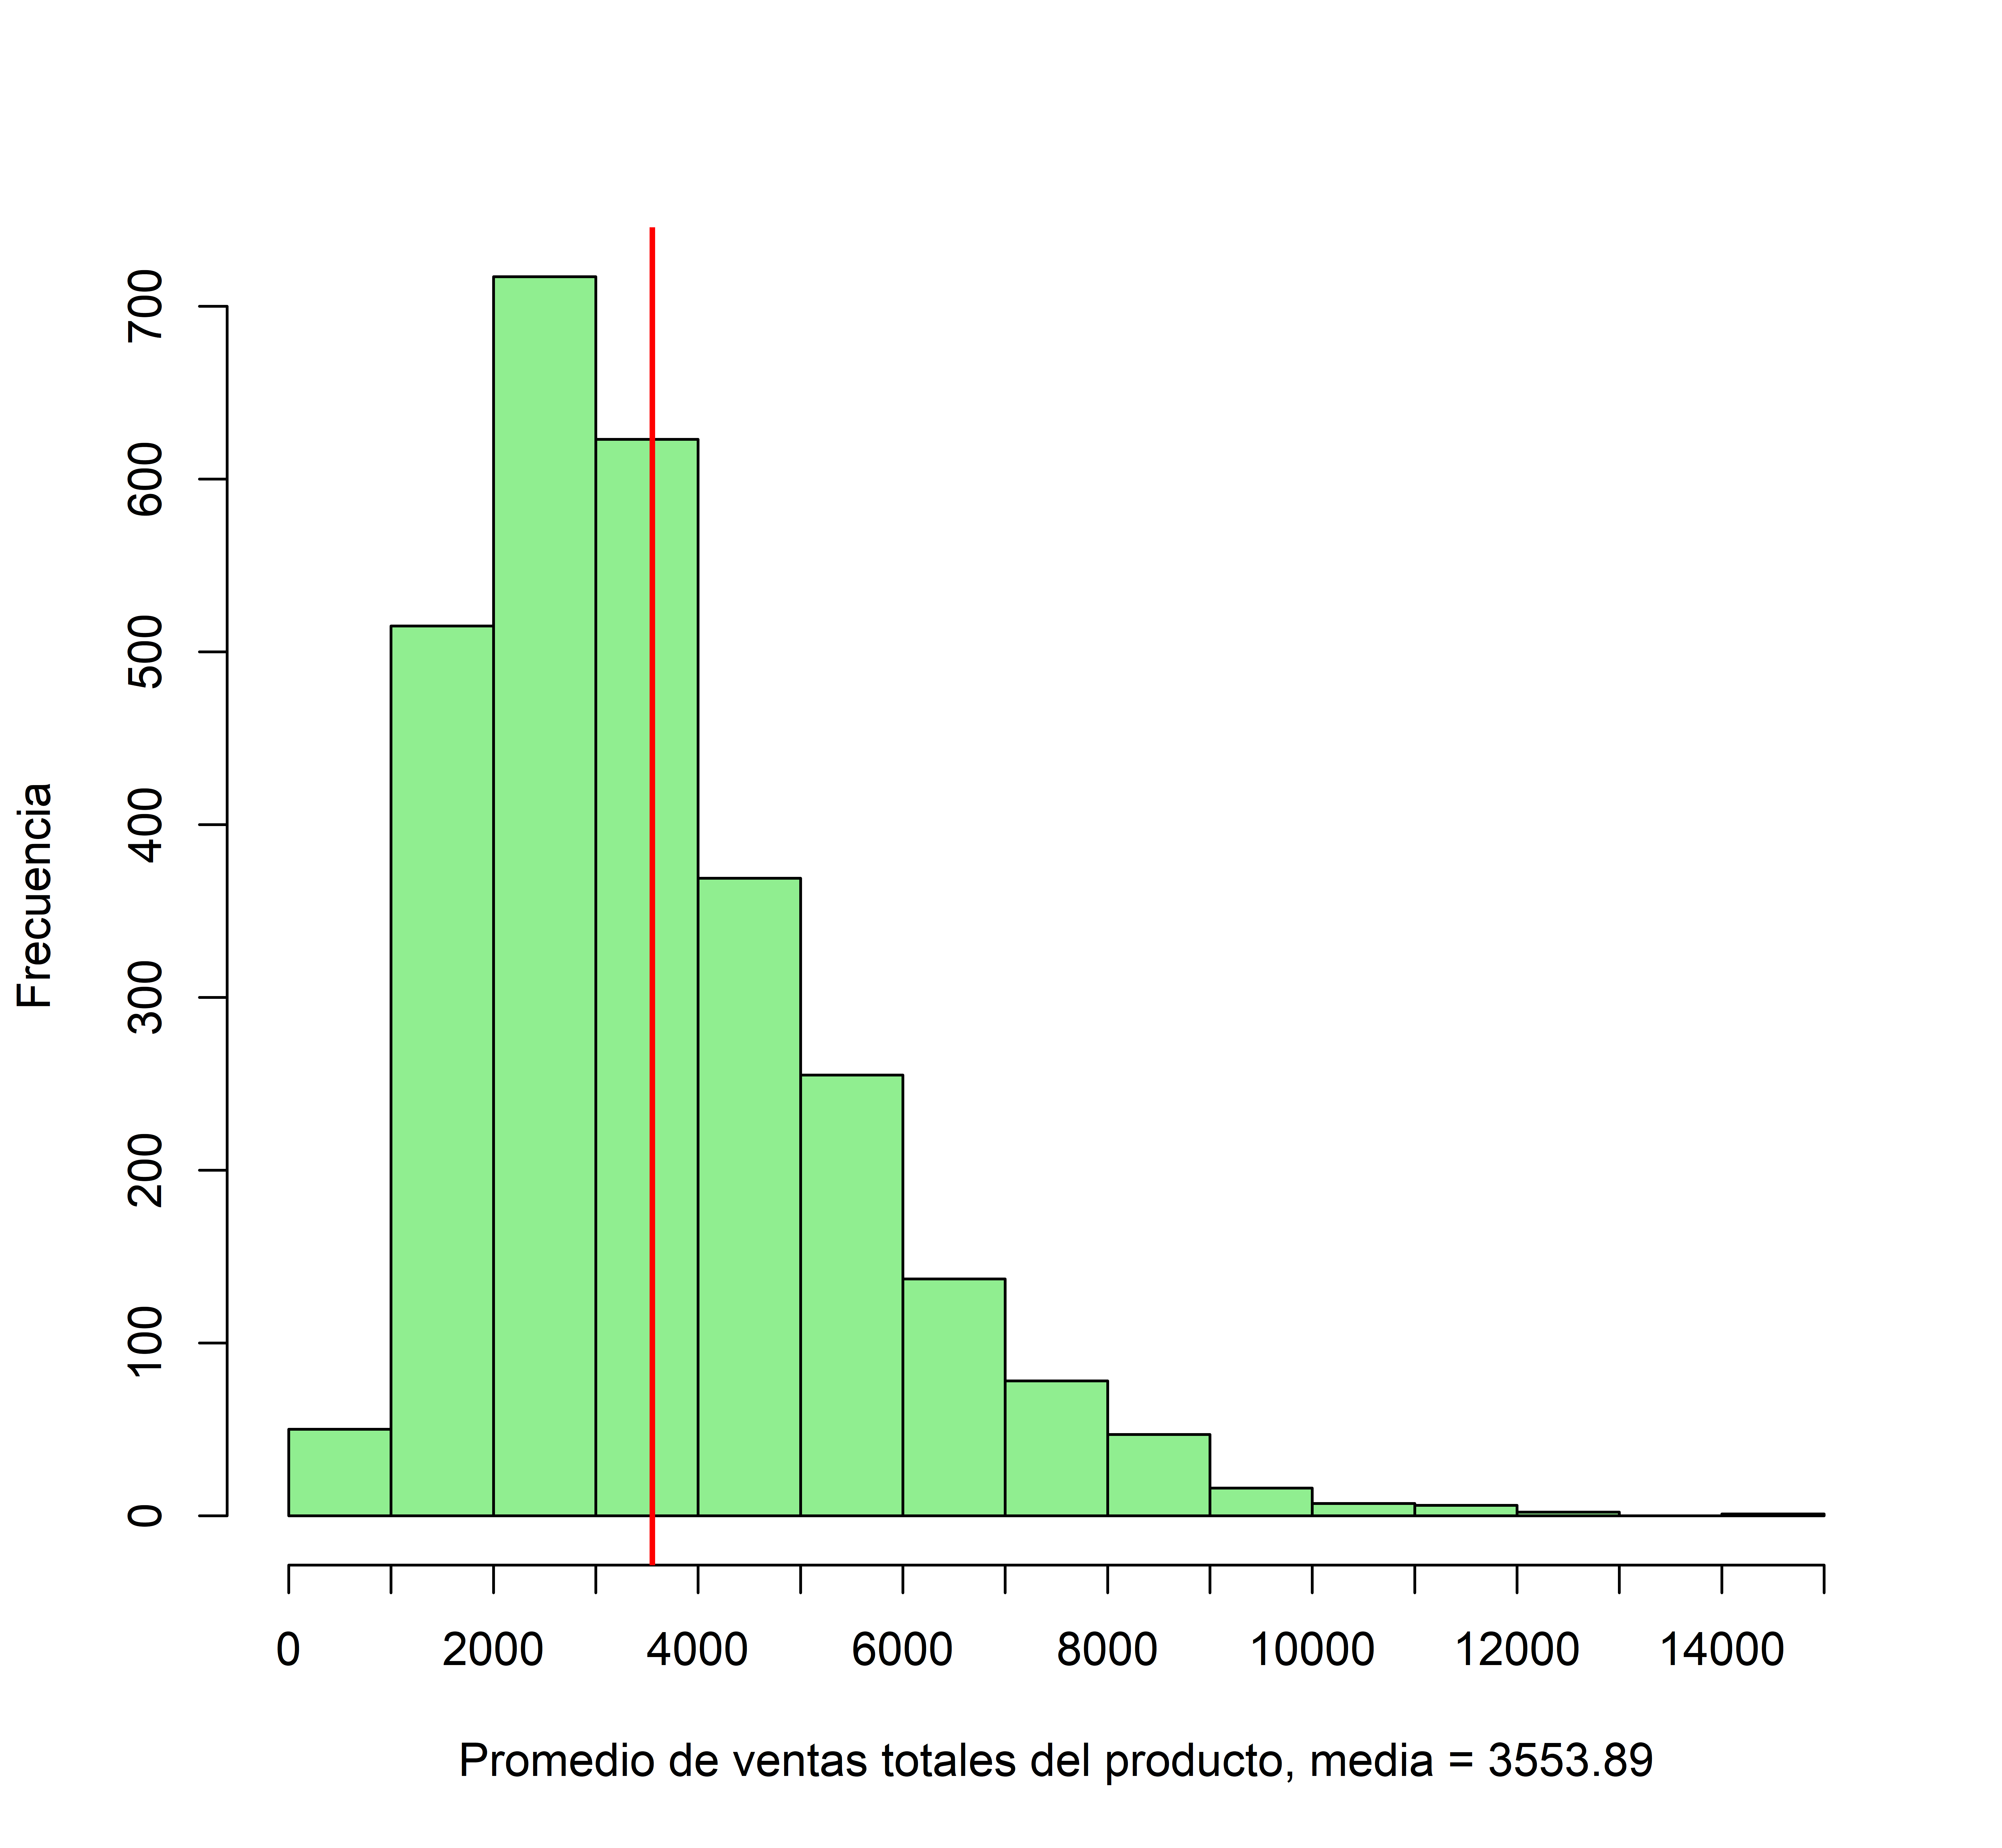
\includegraphics[scale=0.6]{Figures/totalventas.png}
\caption{Histograma de las ventas totales del producto}
\label{inicial}
\end{figure}
    
\begin{figure}[h]
    \begin{center}
    \captionsetup{justification=centering}
    \begin{subfigure}[b]{0.5\textwidth}
        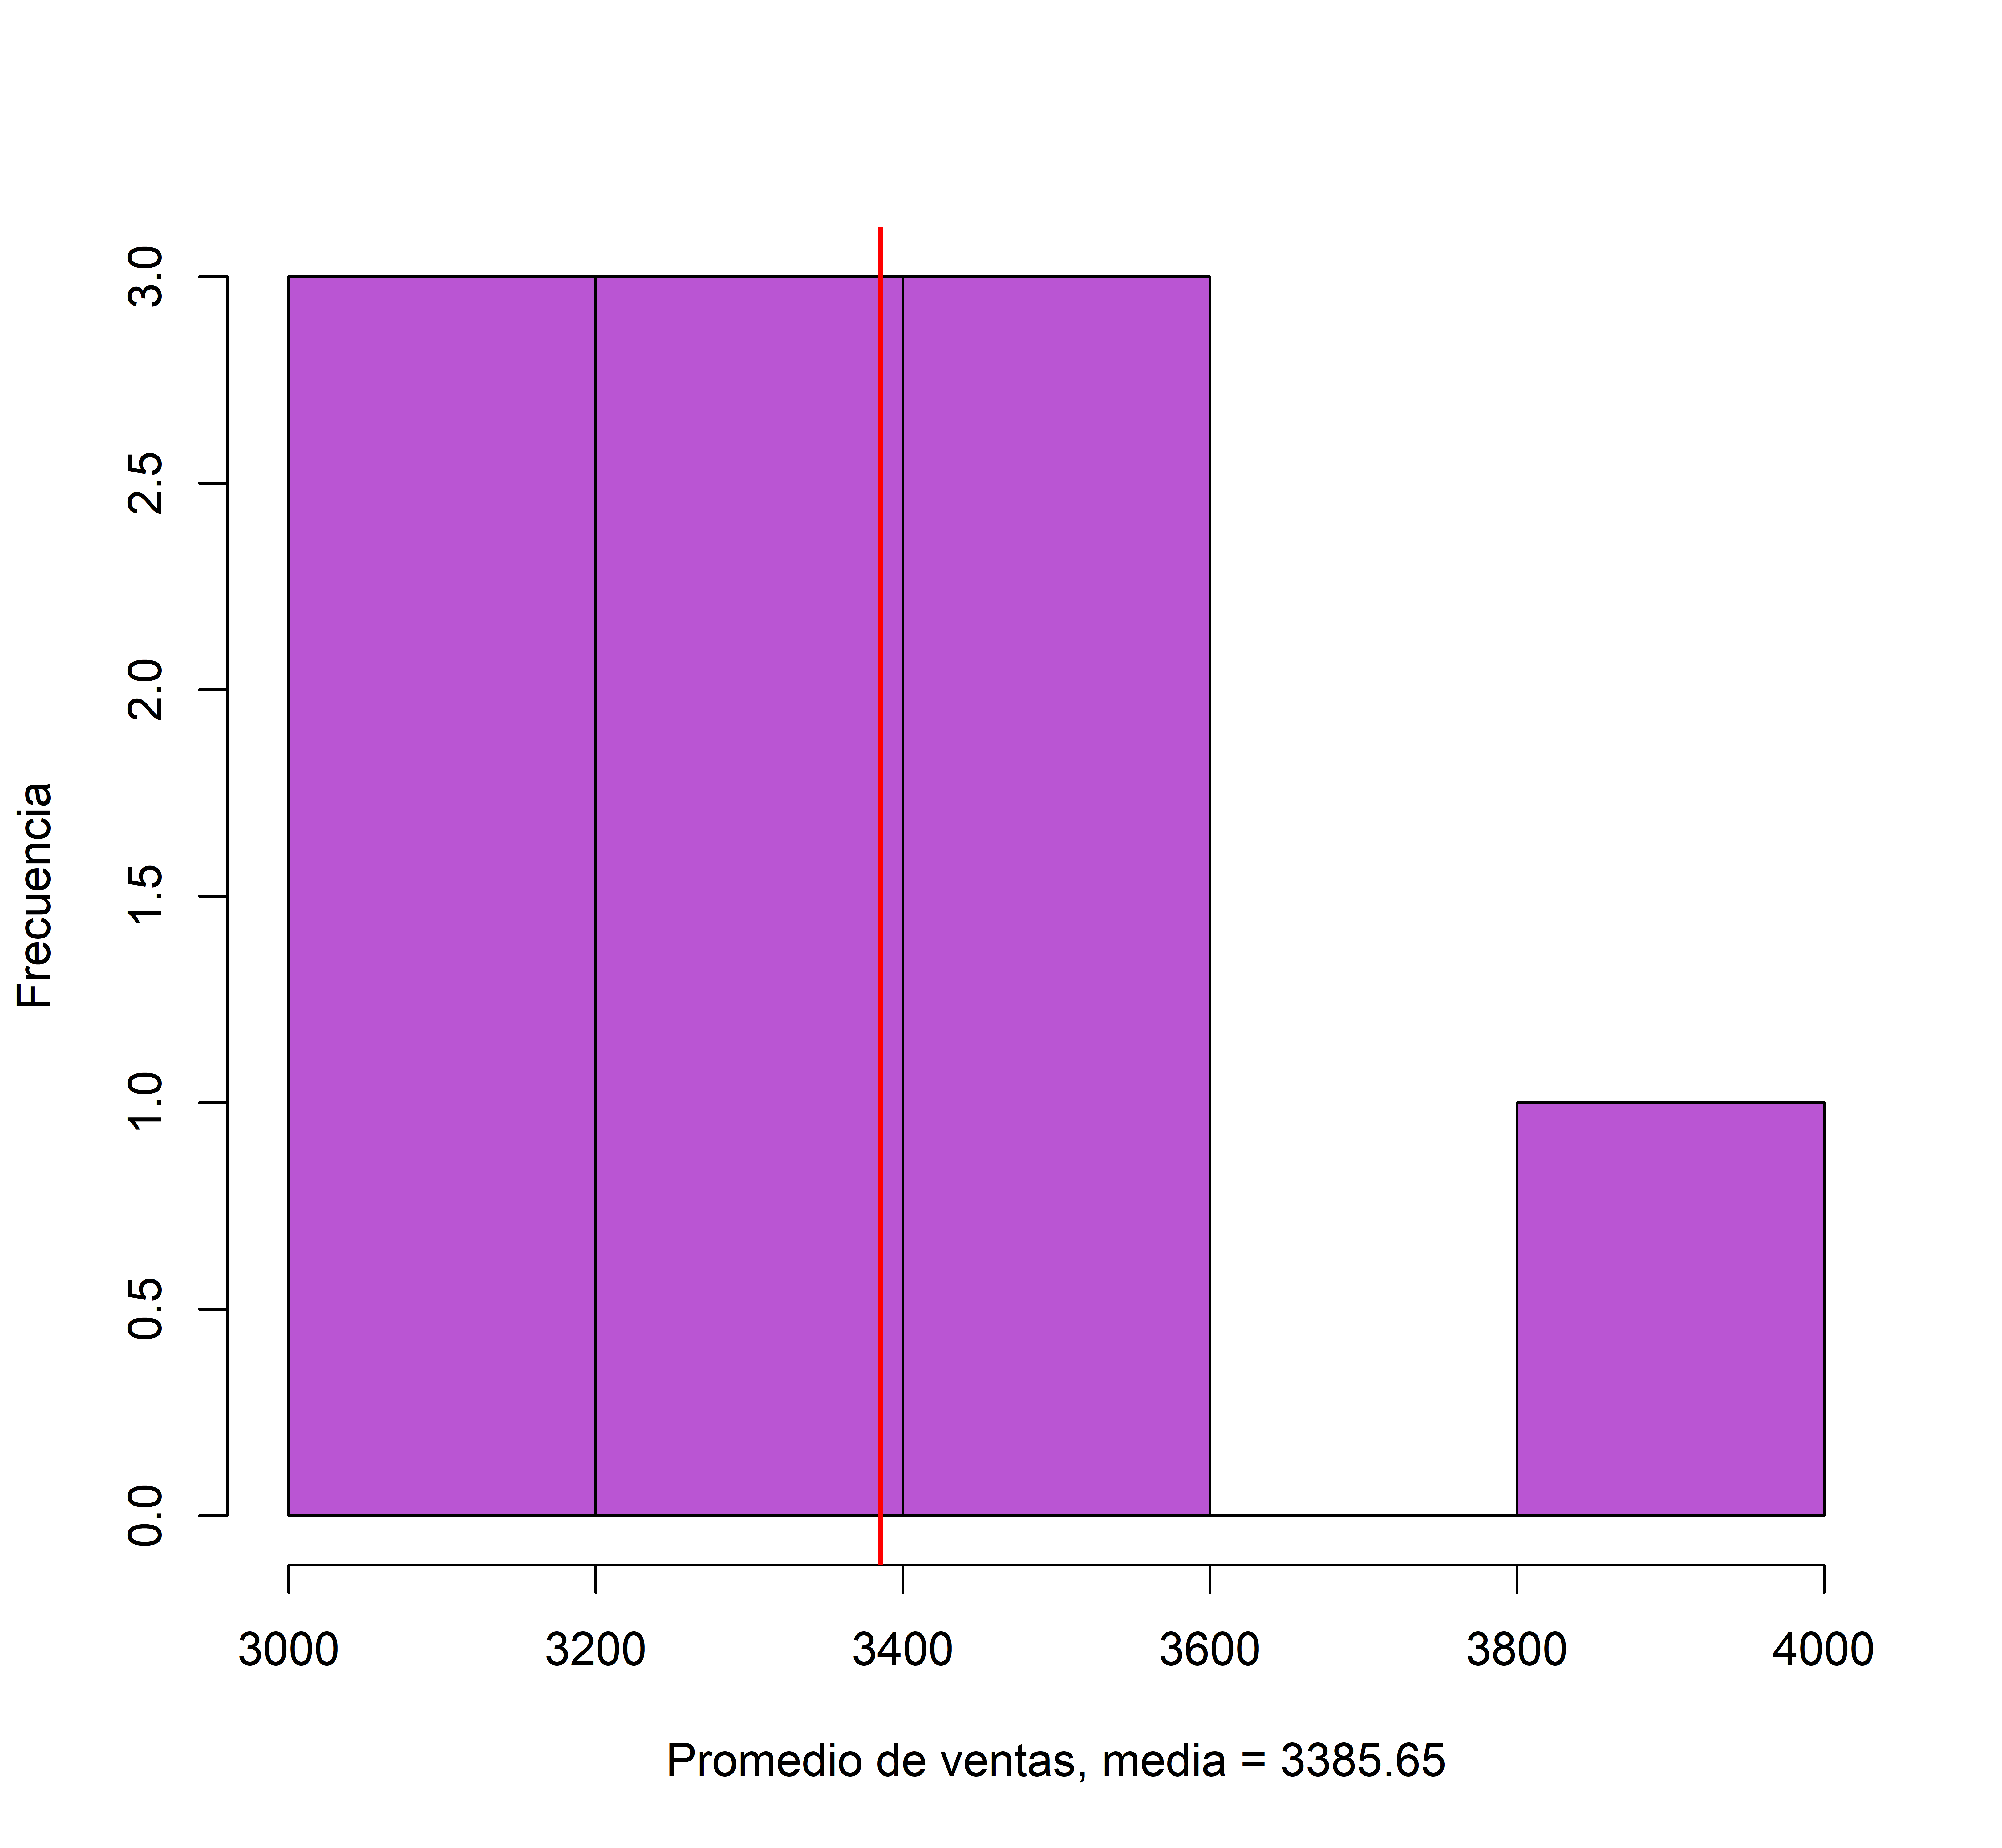
\includegraphics[scale=0.45]{Figures/10-30.png}
        \caption{$n=10$}
    \end{subfigure}
    \begin{subfigure}[b]{0.45\textwidth}
        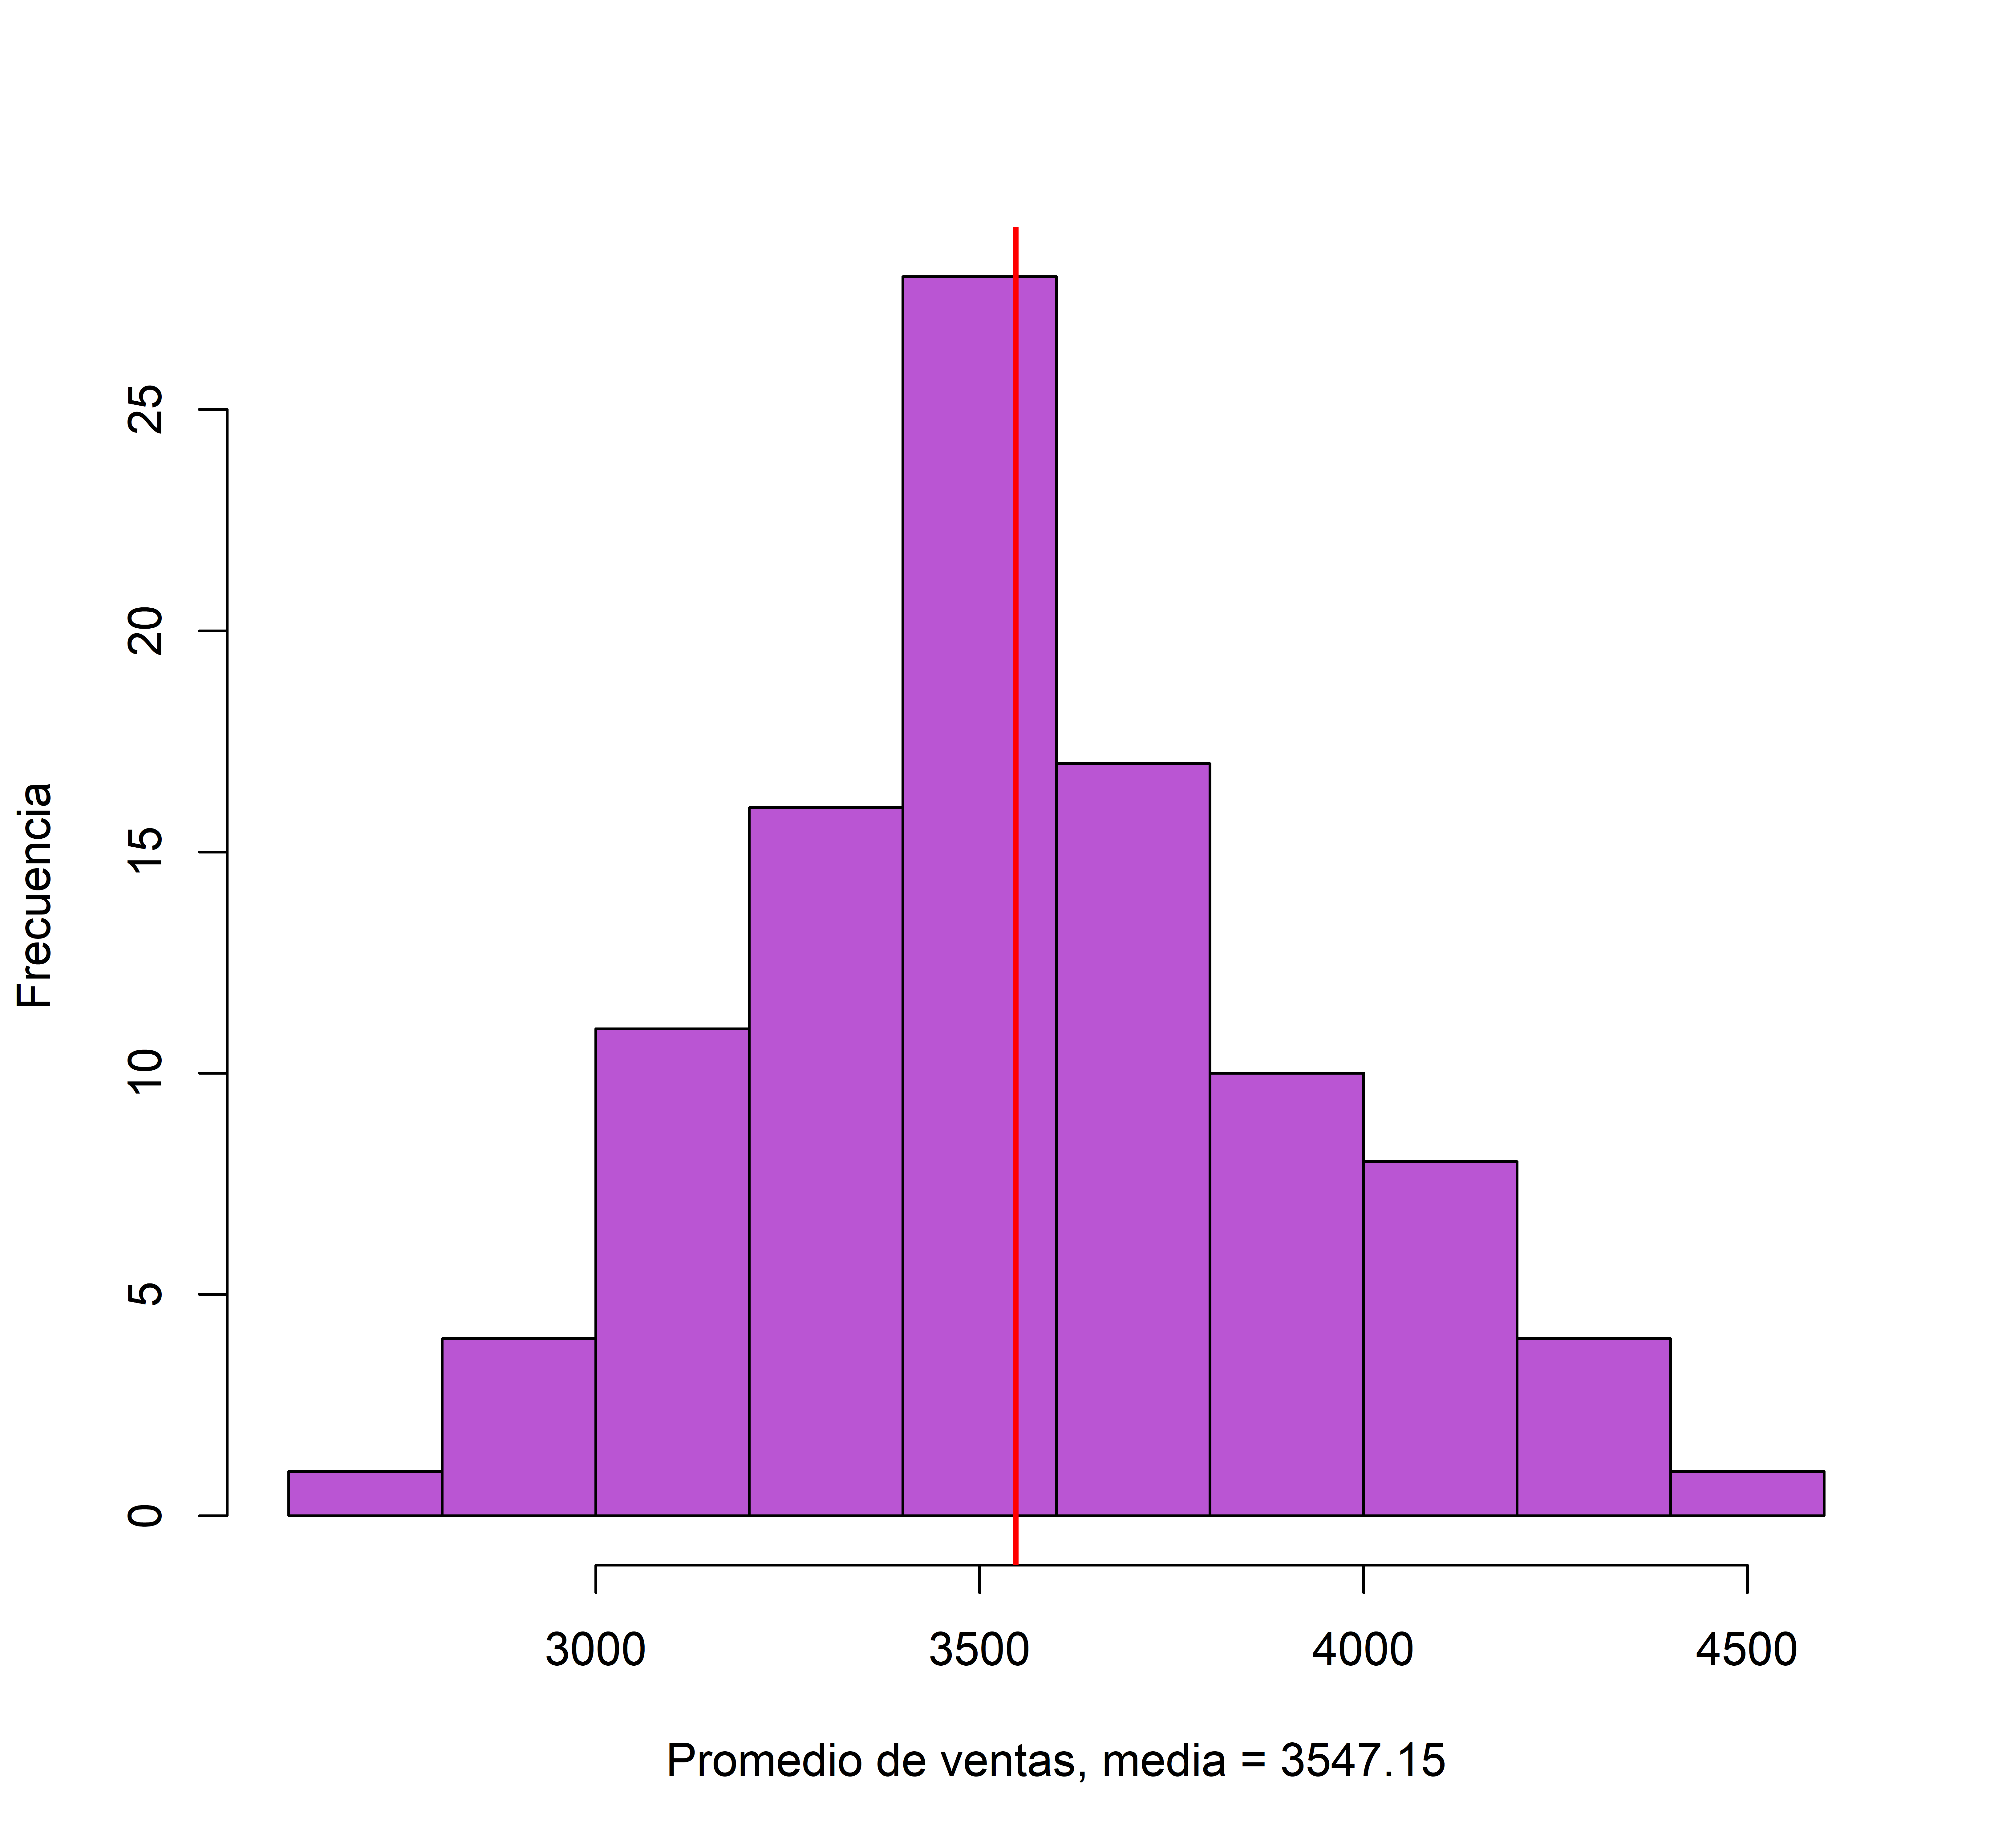
\includegraphics[scale=0.45]{Figures/100-30.png}
        \caption{$n=100$}
    \end{subfigure}
        \begin{subfigure}[b]{0.5\textwidth}
        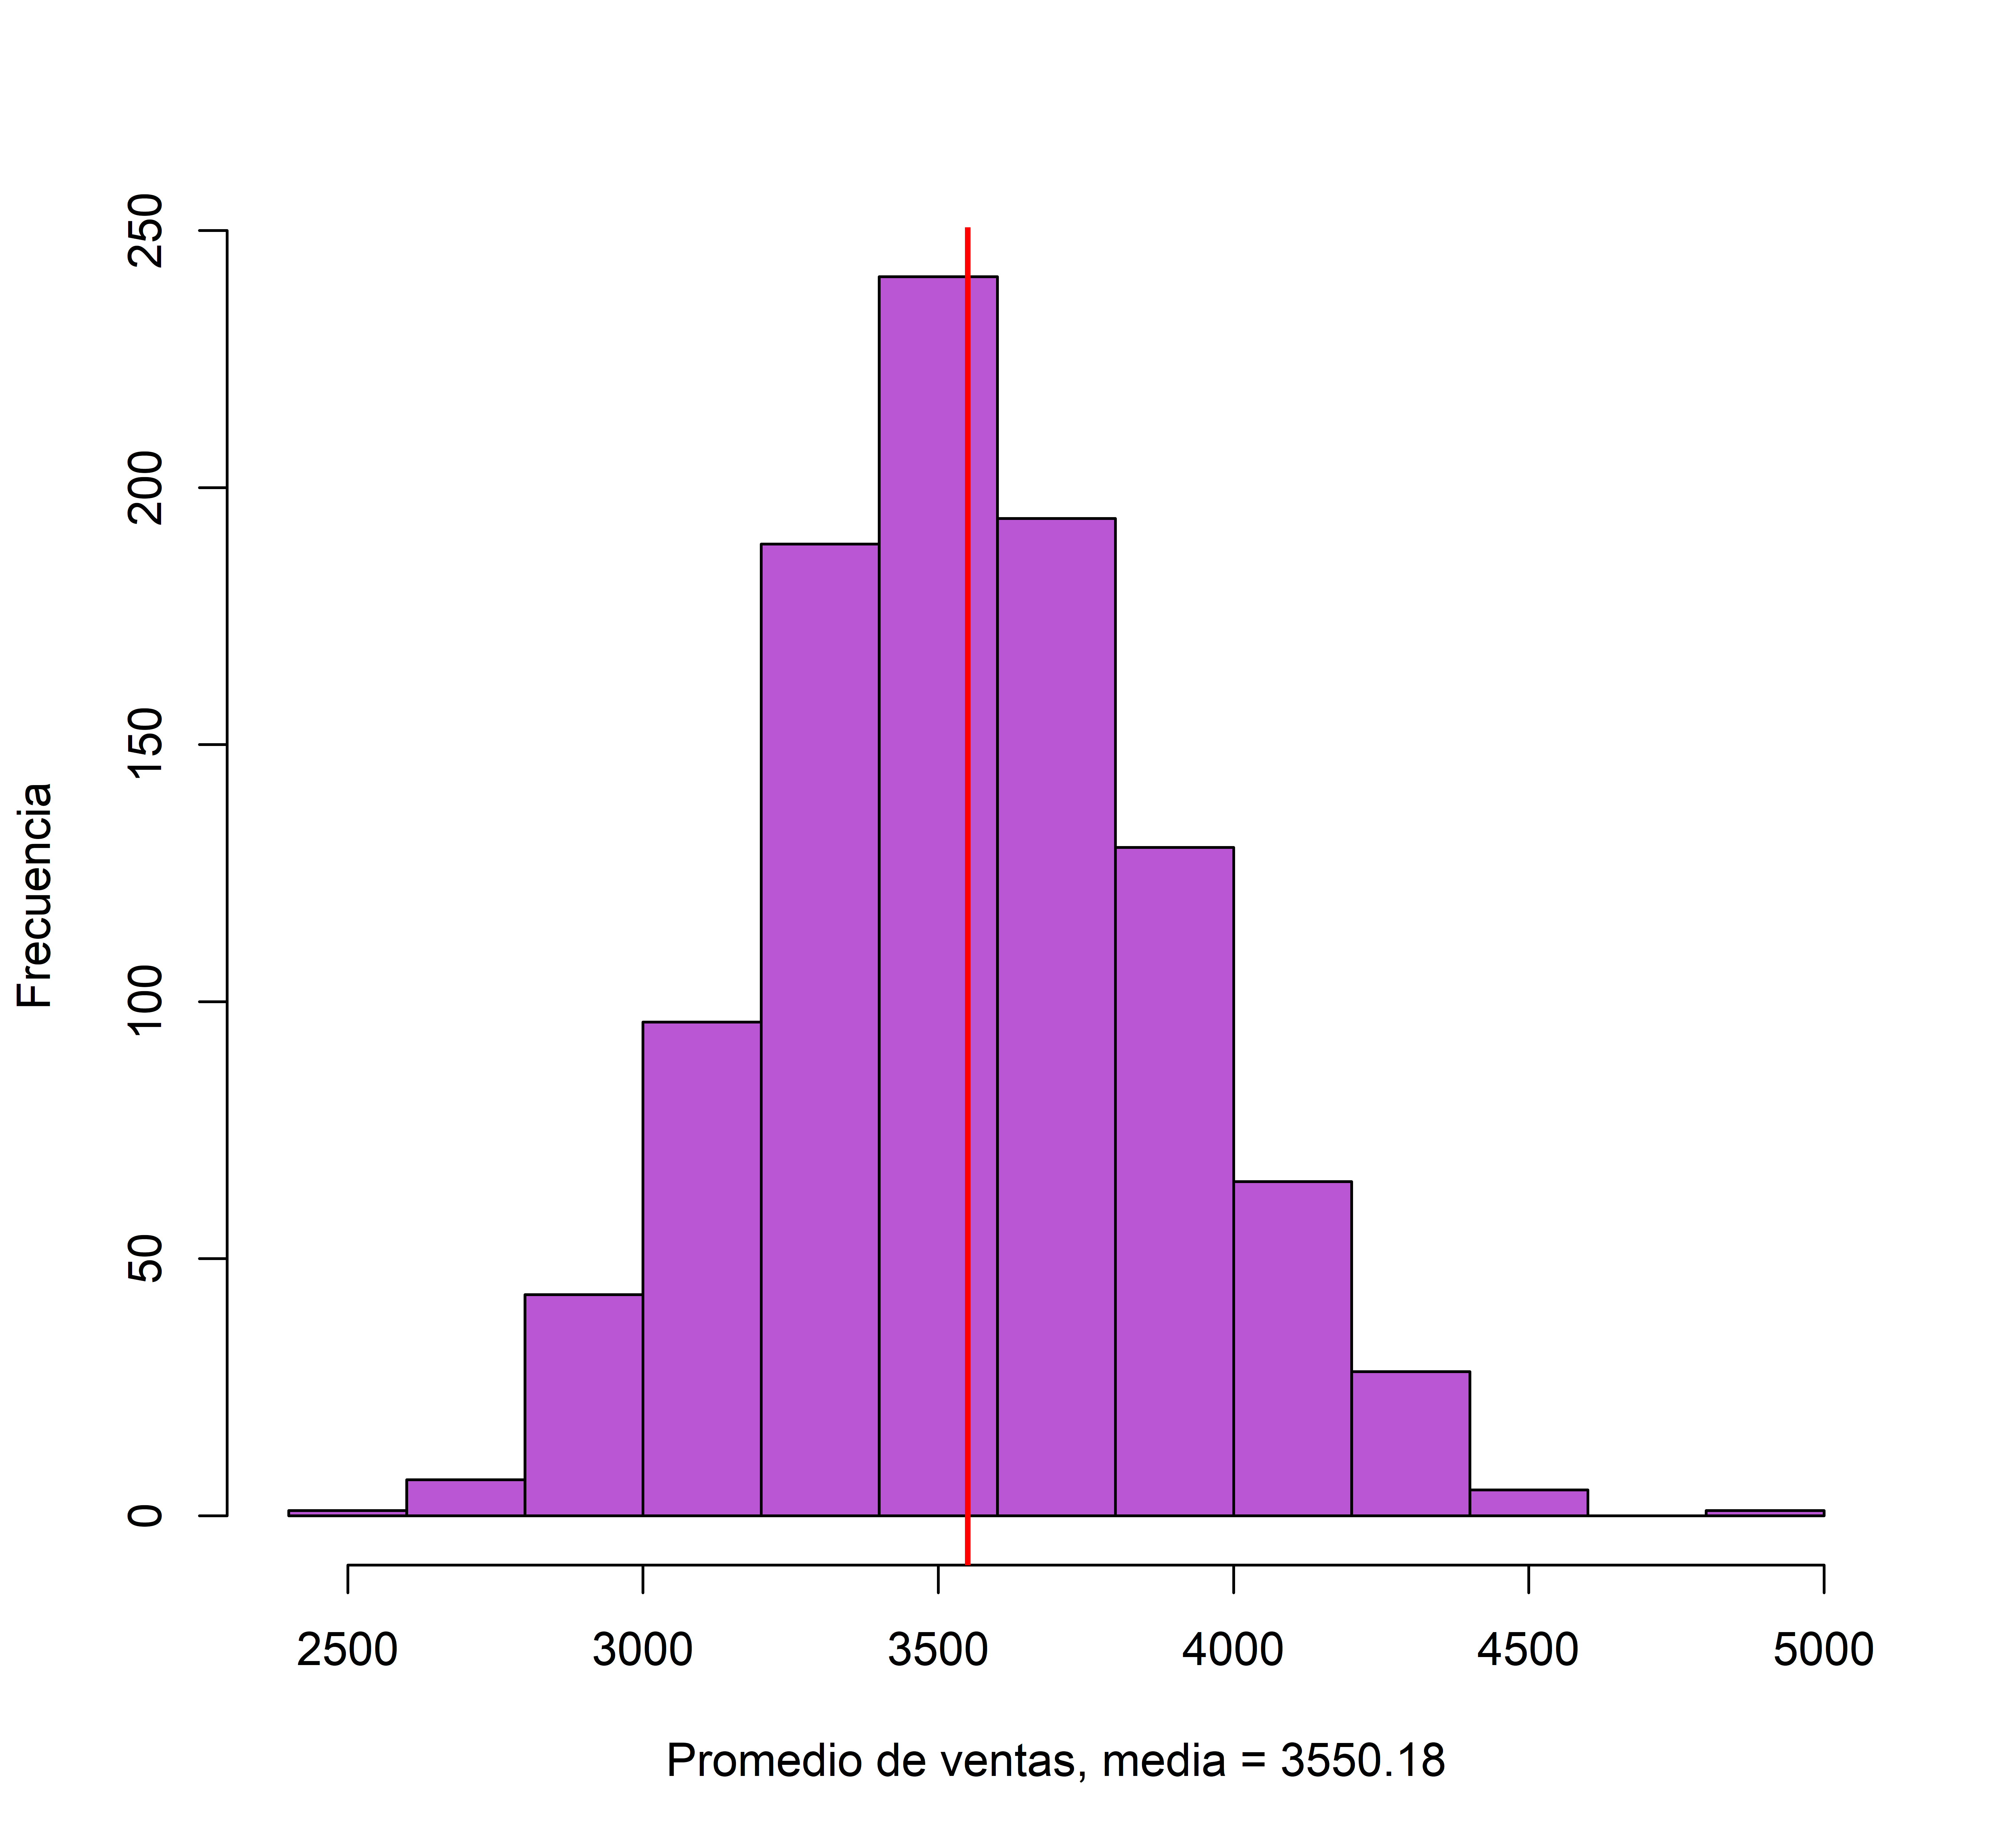
\includegraphics[scale=0.45]{Figures/1000-30.png}
        \caption{$n=1,000$}
    \end{subfigure}
    \begin{subfigure}[b]{0.45\textwidth}
        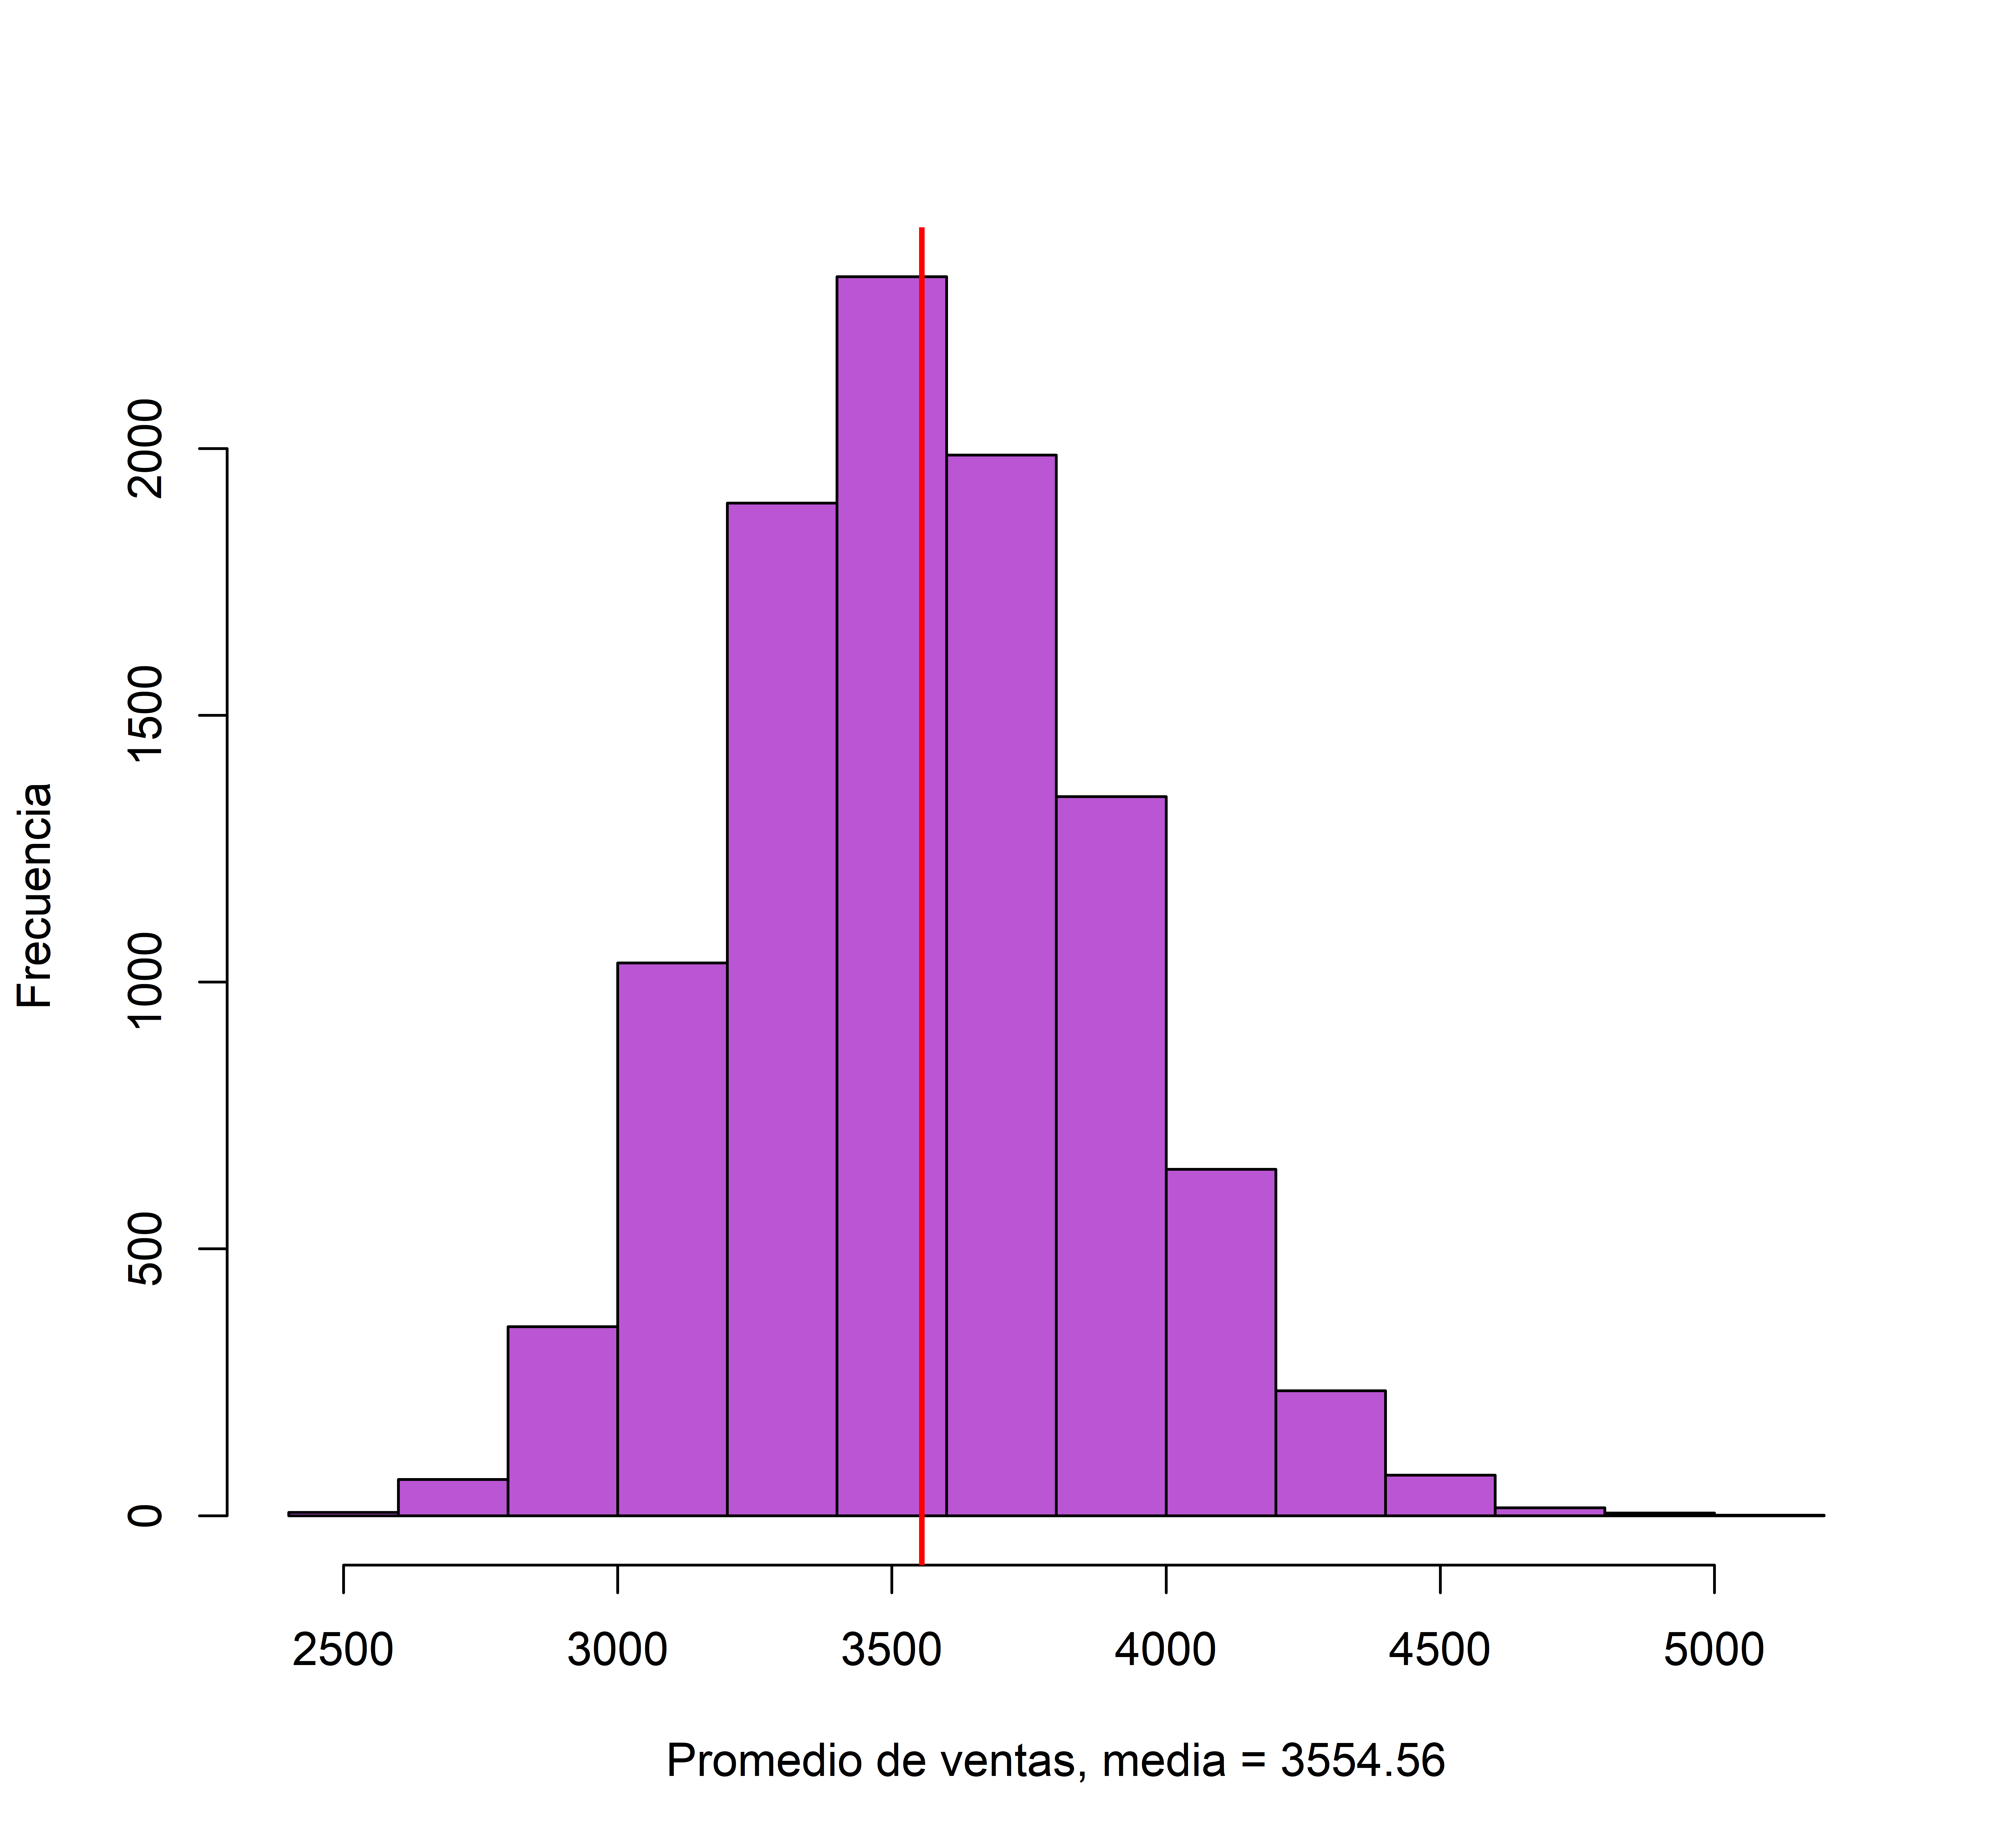
\includegraphics[scale=0.45]{Figures/10000-30.png}
        \caption{$n=10,000$}
    \end{subfigure}
    \caption{Resultados de la experimentación con $n$ muestras de tamaño $30$}
    \label{con30}
    \end{center}
\end{figure}

\begin{figure}[h]
    \begin{center}
    \captionsetup{justification=centering}
    \begin{subfigure}[b]{0.5\textwidth}
        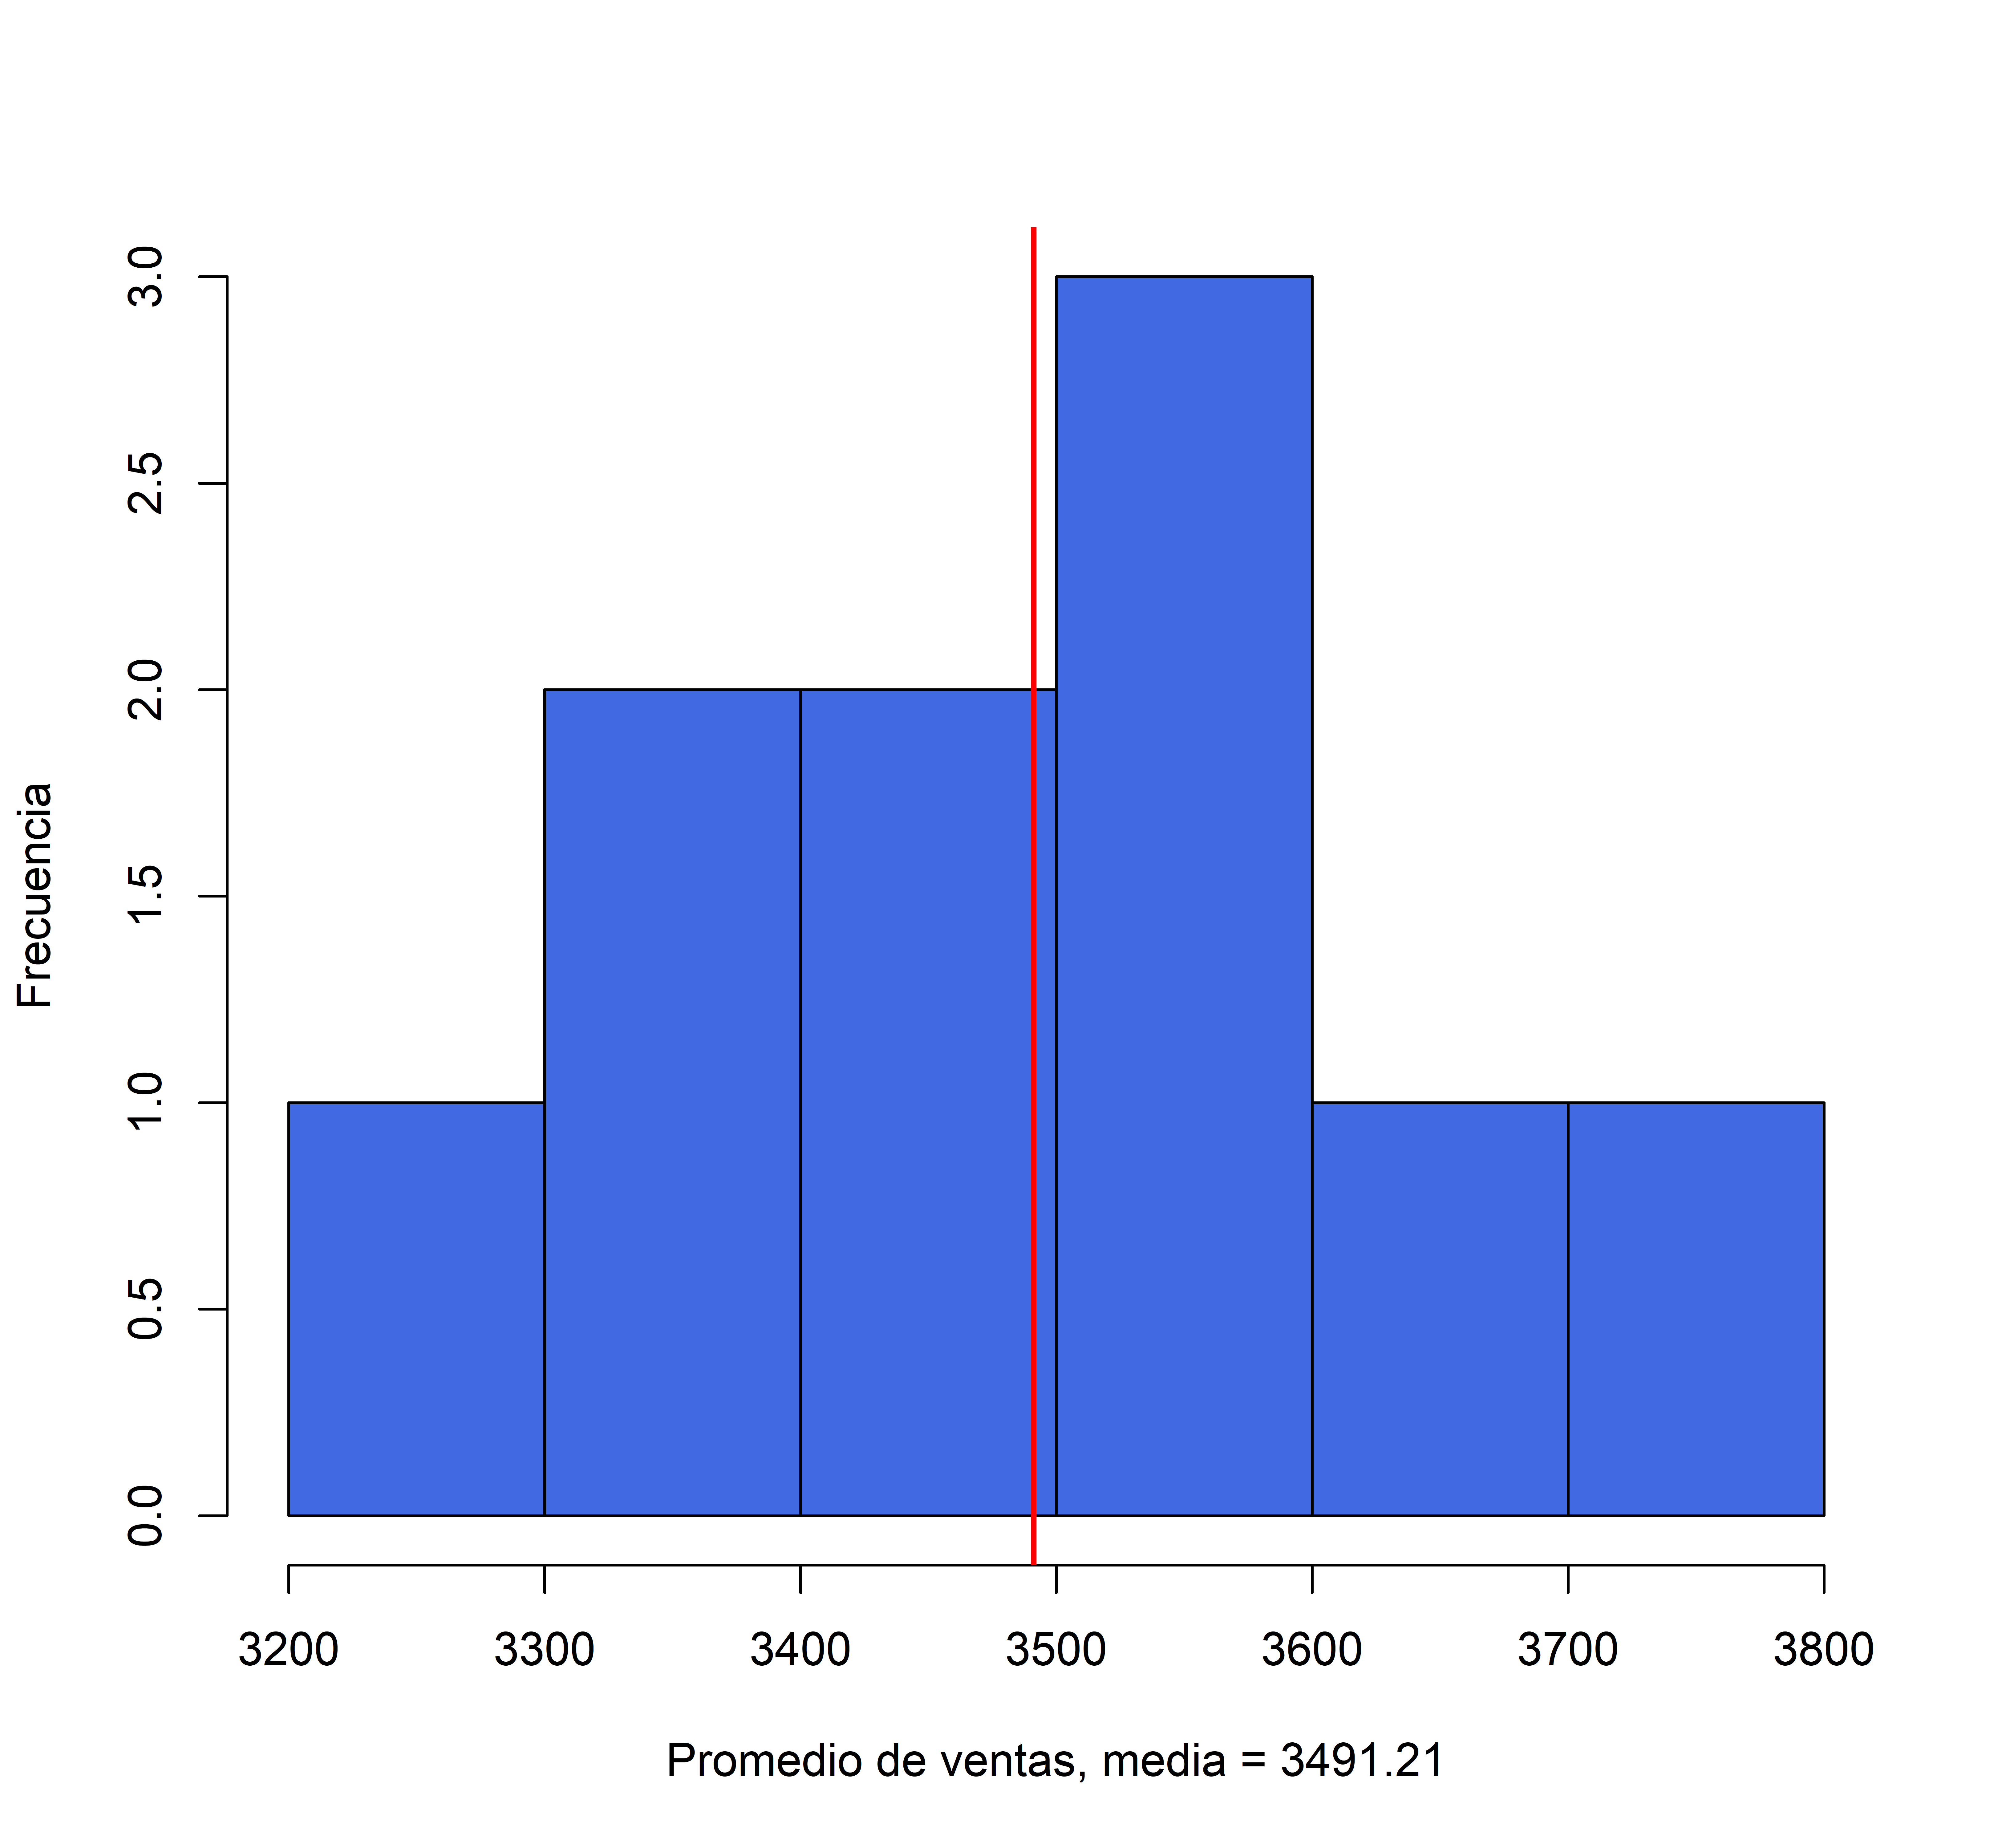
\includegraphics[scale=0.45]{Figures/10-100.png}
        \caption{$n=10$}
    \end{subfigure}
    \begin{subfigure}[b]{0.45\textwidth}
        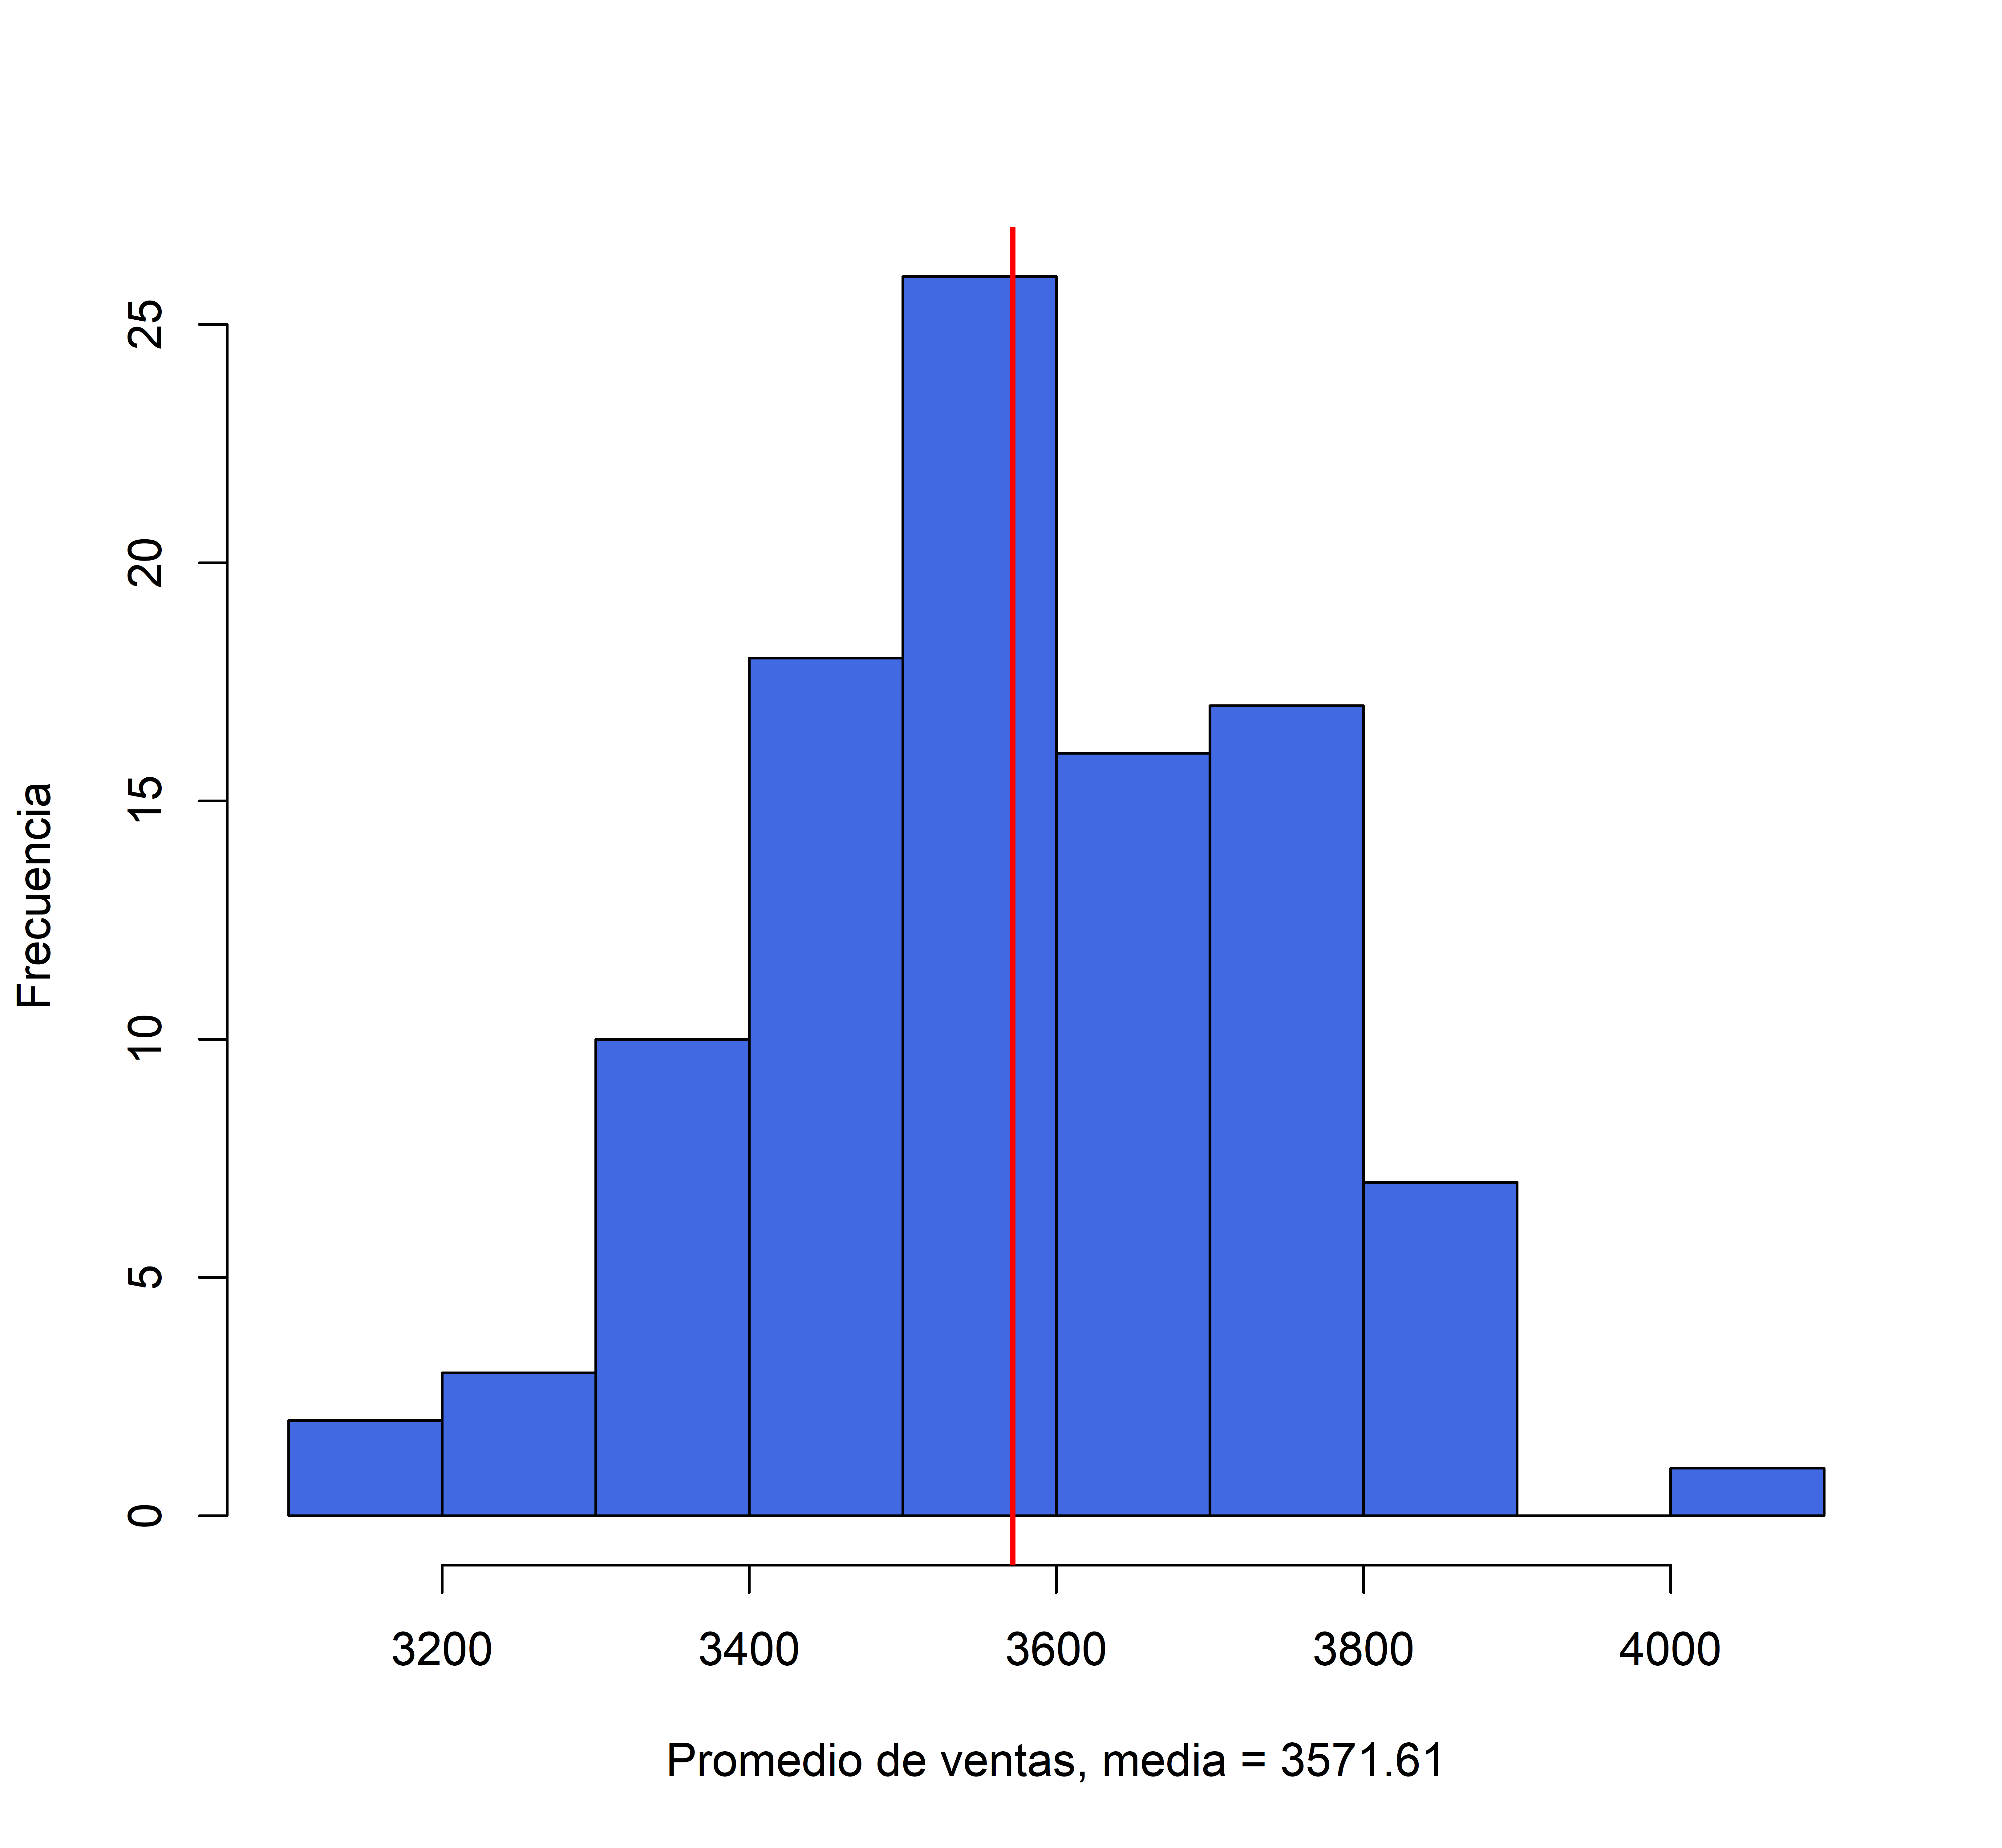
\includegraphics[scale=0.45]{Figures/100-100.png}
        \caption{$n=100$}
    \end{subfigure}
        \begin{subfigure}[b]{0.5\textwidth}
        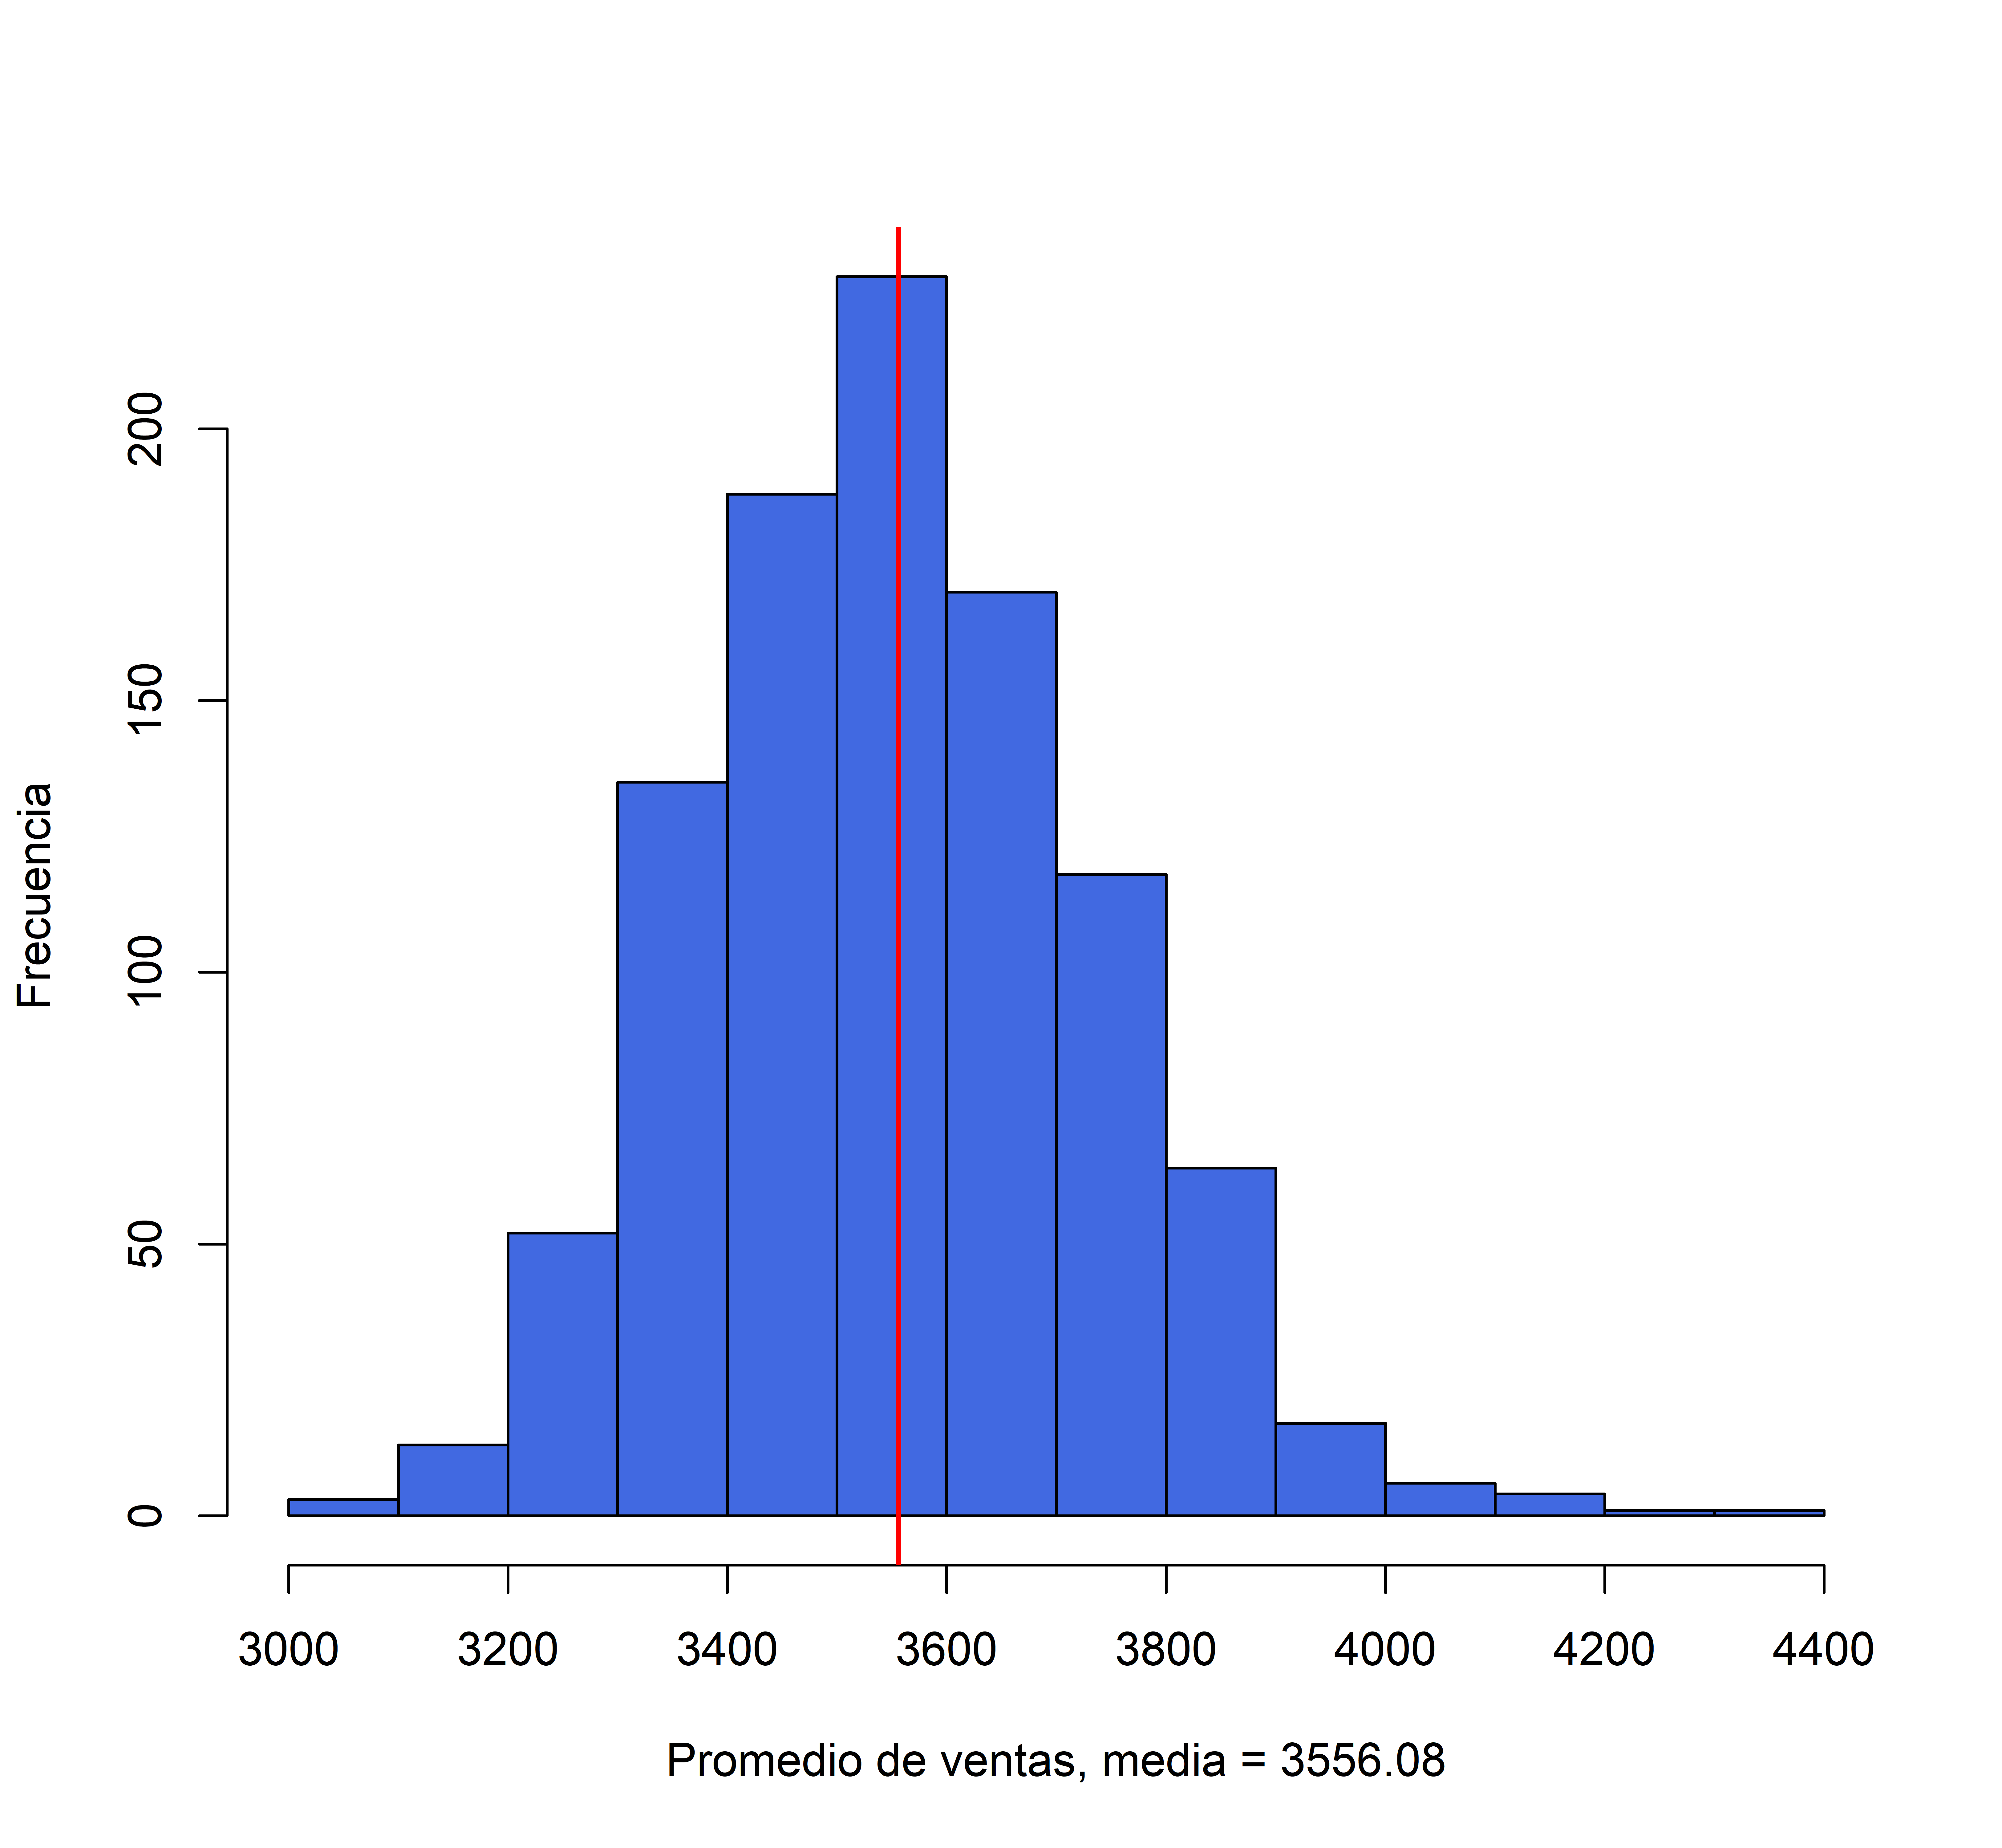
\includegraphics[scale=0.45]{Figures/1000-100.png}
        \caption{$n=1,000$}
    \end{subfigure}
    \begin{subfigure}[b]{0.45\textwidth}
        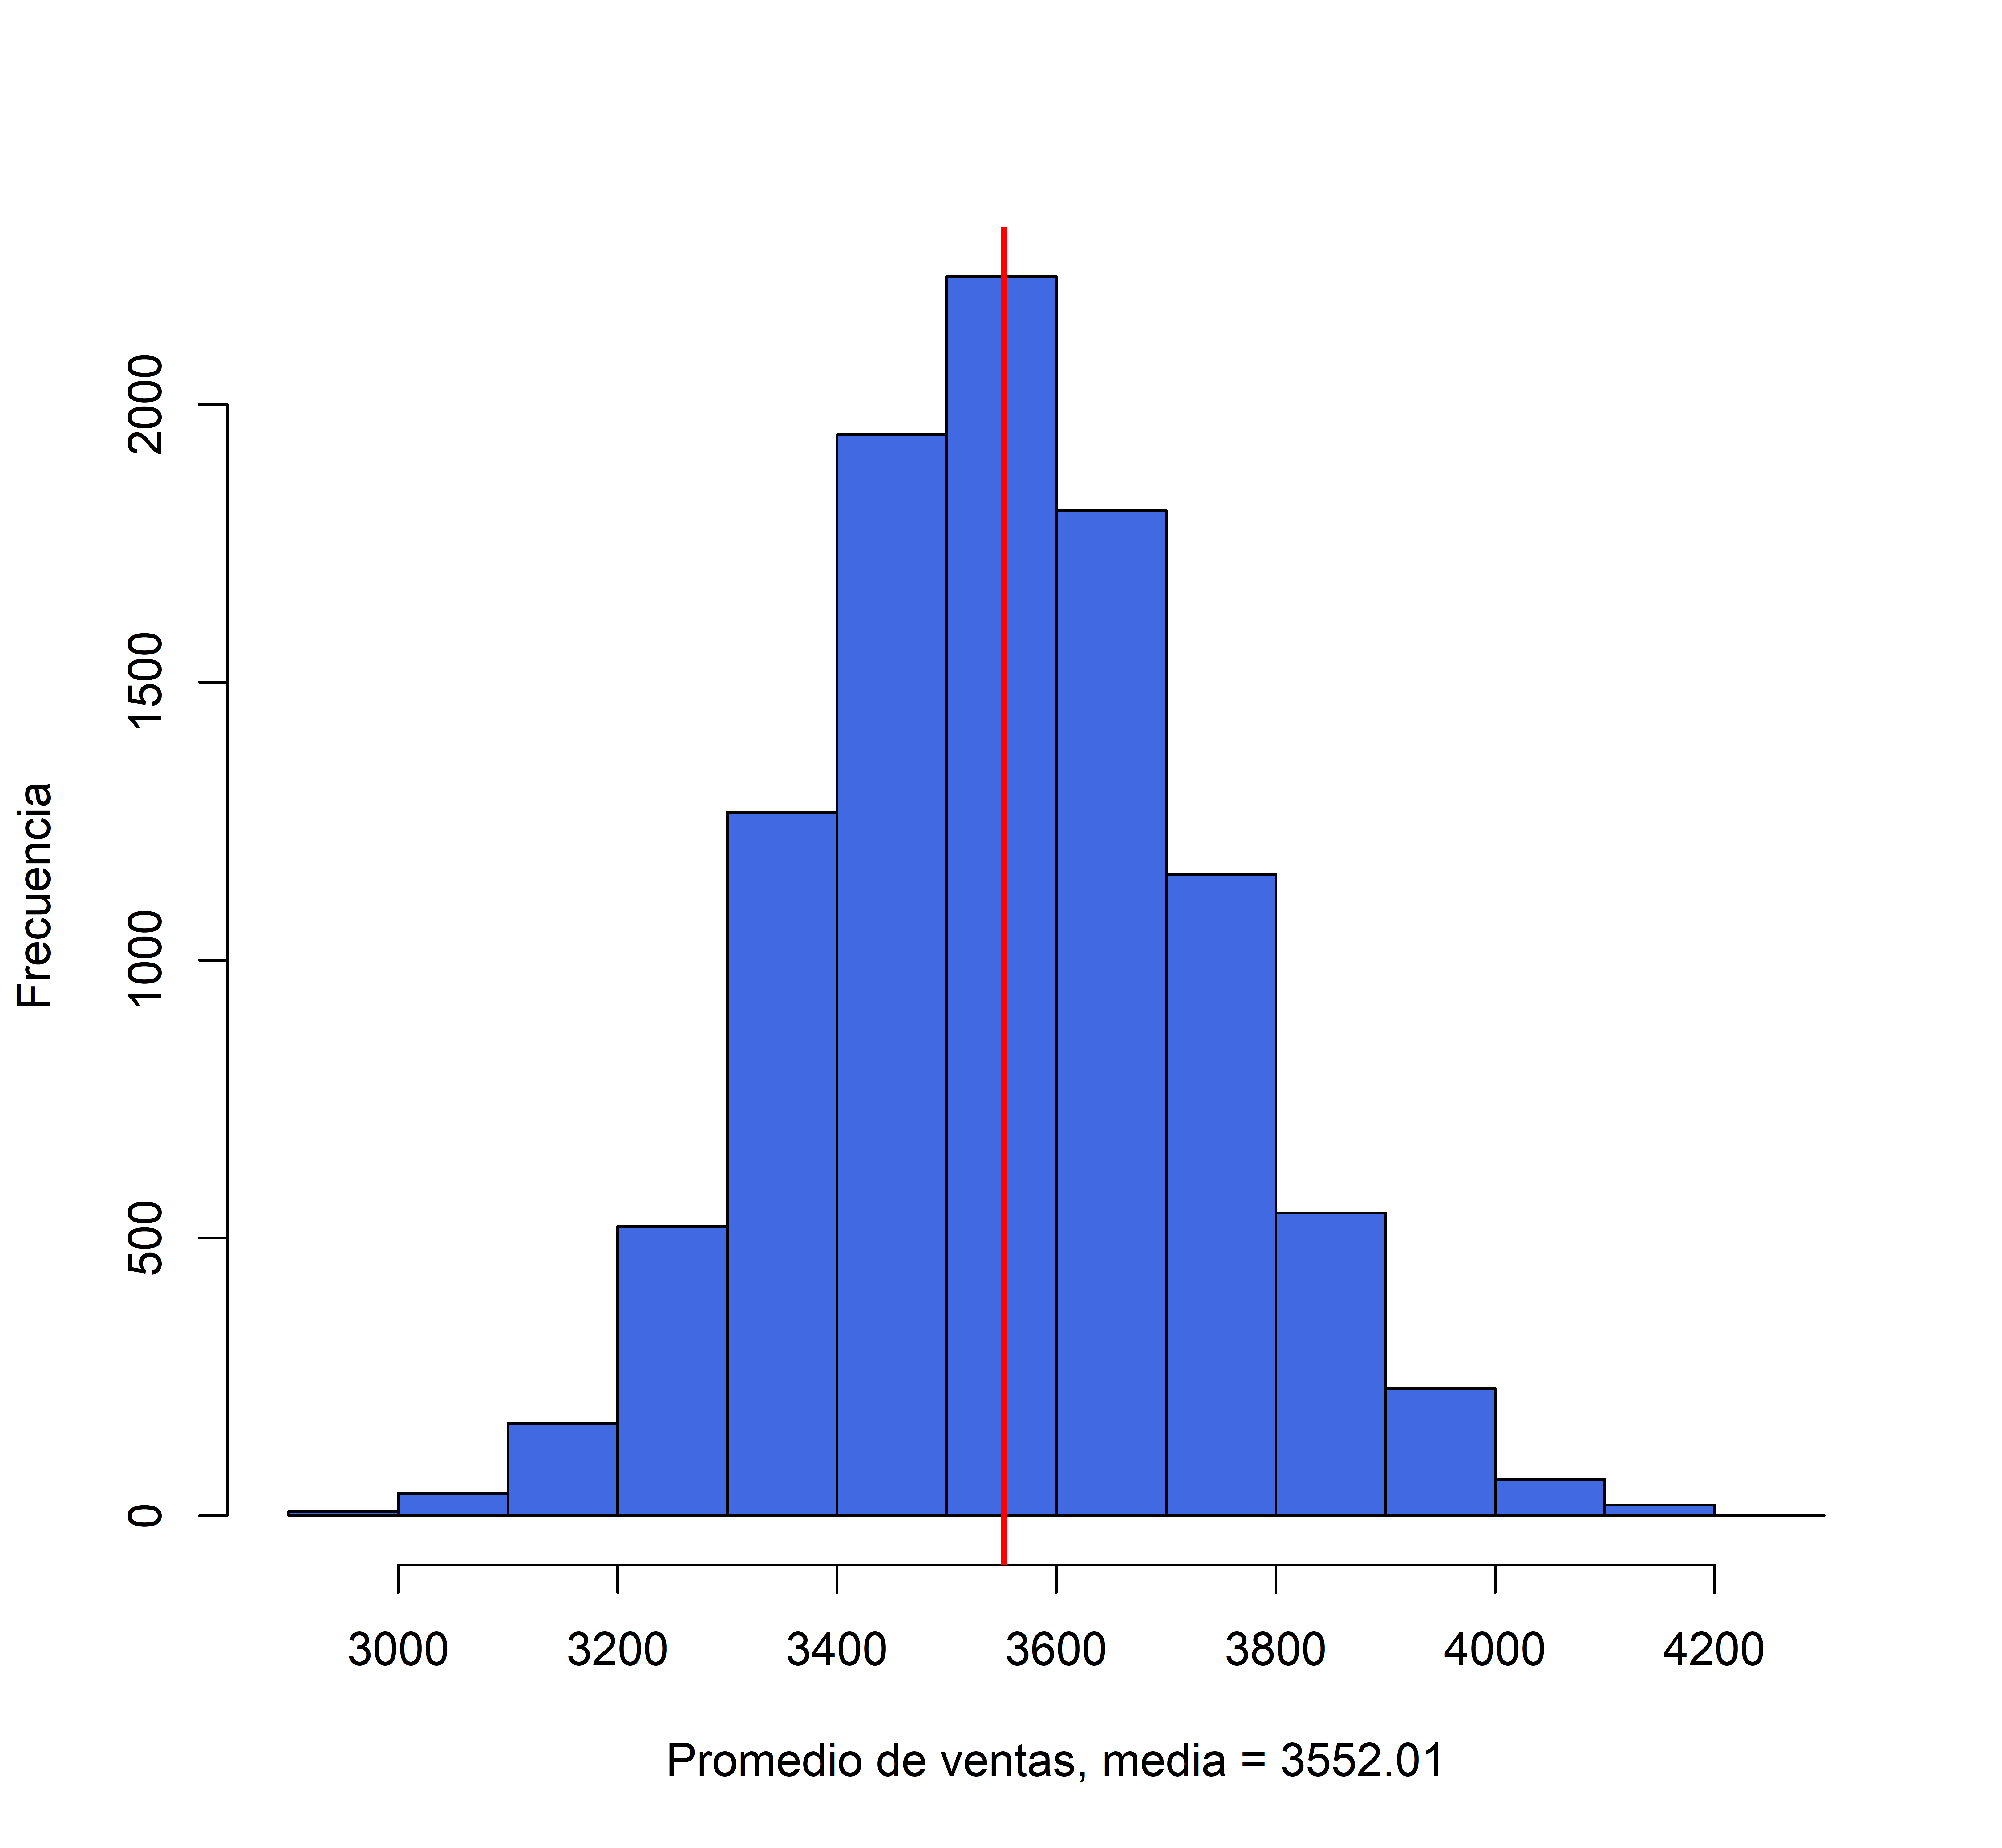
\includegraphics[scale=0.45]{Figures/10000-100.png}
        \caption{$n=10,000$}
    \end{subfigure}
    \caption{Resultados de la experimentación con $n$ muestras de tamaño $100$}
    \label{con100}
    \end{center}
\end{figure}

\bibliography{refProbabilidad}
\bibliographystyle{plain}

\end{document}

